% ============================================================
%  Hybrid Cyber Attack Prediction Platform -- Group 14, CEK
%  B.Tech Final-Year Project Review -- Complete Technical Presentation
%  Architecture: Hybrid GAT + GRU + VGAE Provenance Graph Threat Detection Framework
%  Primary Benchmark: DARPA Transparent Computing (TC E3/E5)
%  Compile: pdflatex main.tex  (run twice for cross-references)
% ============================================================
\documentclass[aspectratio=169,10pt]{beamer}
\usetheme{Madrid}
\usecolortheme{default}
\usefonttheme{professionalfonts}
\usepackage[T1]{fontenc}
\usepackage{lmodern}
\usepackage{amsmath,amssymb}
\usepackage{booktabs}
\usepackage{tikz}
\usepackage{tabularx}
\usepackage{colortbl}
\usepackage{ragged2e}
\usepackage{array}
\usepackage{multirow}
\usetikzlibrary{arrows.meta,positioning,fit,backgrounds,calc,shadows,shapes.geometric}

% ---- TABLE COLUMN TYPES -----------------------------------------------
\newcolumntype{L}[1]{>{\raggedright\arraybackslash}p{#1}}
\newcolumntype{C}[1]{>{\centering\arraybackslash}p{#1}}
\newcolumntype{R}[1]{>{\raggedleft\arraybackslash}p{#1}}
\newcolumntype{Y}{>{\raggedright\arraybackslash}X}

% ---- COLOUR PALETTE ---------------------------------------------------
\definecolor{prismNavy}{RGB}{13,29,54}
\definecolor{prismBlue}{RGB}{38,126,190}
\definecolor{prismTeal}{RGB}{28,161,157}
\definecolor{prismMint}{RGB}{224,247,242}
\definecolor{prismGold}{RGB}{229,166,50}
\definecolor{rowA}{RGB}{240,248,255}
\definecolor{rowB}{RGB}{255,255,255}
\definecolor{strengthGreen}{RGB}{0,120,60}
\definecolor{limitRed}{RGB}{180,0,0}
\definecolor{codeBg}{RGB}{245,247,250}

% ---- BEAMER COLOURS ---------------------------------------------------
\setbeamercolor{structure}{fg=prismBlue}
\setbeamercolor{frametitle}{bg=prismNavy,fg=white}
\setbeamercolor{block title}{bg=prismBlue,fg=white}
\setbeamercolor{block body}{bg=prismMint,fg=black}
\setbeamertemplate{navigation symbols}{}
\setbeamercolor{author in head/foot}{bg=prismNavy,fg=white}
\setbeamercolor{title in head/foot}{bg=prismBlue,fg=white}
\setbeamercolor{date in head/foot}{bg=prismNavy,fg=white}
\setbeamertemplate{itemize item}{\color{prismTeal}$\blacktriangleright$}
\setbeamertemplate{itemize subitem}{\color{prismBlue}$\triangleright$}
\setbeamersize{text margin left=0.45cm,text margin right=0.45cm}

% ---- FOOTLINE ---------------------------------------------------------
\setbeamertemplate{footline}{%
  \leavevmode\hbox{%
  \begin{beamercolorbox}[wd=.333333\paperwidth,ht=2.25ex,dp=1ex,center]{author in head/foot}%
    \usebeamerfont{author in head/foot}Group 14 (CEK)\end{beamercolorbox}%
  \begin{beamercolorbox}[wd=.333333\paperwidth,ht=2.25ex,dp=1ex,center]{title in head/foot}%
    \usebeamerfont{title in head/foot}B.Tech Final-Year Project Review\end{beamercolorbox}%
  \begin{beamercolorbox}[wd=.333333\paperwidth,ht=2.25ex,dp=1ex,right]{date in head/foot}%
    \usebeamerfont{date in head/foot}\insertdate\hspace*{2em}\insertframenumber{}/\inserttotalframenumber\hspace*{2ex}\end{beamercolorbox}}%
  \vskip0pt}

% ---- FRAMETITLE -------------------------------------------------------
\setbeamertemplate{frametitle}{%
  \nointerlineskip%
  \begin{beamercolorbox}[wd=\paperwidth,ht=1.20cm,dp=0pt,leftskip=0.45cm,rightskip=0.45cm]{frametitle}%
    \vbox to 1.20cm{%
      \vfill%
      \raggedright\fontsize{9.2pt}{11.0pt}\selectfont\textbf{\insertframetitle}%
      \vfill%
    }%
  \end{beamercolorbox}%
}

% ---- DOCUMENT METADATA ------------------------------------------------
\title[Cyber Attack Prediction Platform]{CYBER ATTACK PREDICTION PLATFORM USING SPATIO-TEMPORAL GRAPH NEURAL NETWORKS}
\subtitle{A Hybrid GAT + GRU + VGAE Provenance Graph Architecture for Real-Time Threat Detection, Causal Investigation \& MITRE ATT\&CK Reconstruction}
\author{Muhammed Nasih K P \and Sumayya Ershad \and Najmunniza N \and K.S.\ Mahadev}
\institute{Dept.\ of Computer Science \& Engineering, College of Engineering, Karunagappally}
\date{October 2026}

% ---- HELPER COMMANDS --------------------------------------------------
\newcommand{\lrhdr}{%
  \rowcolor{prismNavy}%
  {\scriptsize\textcolor{white}{\textbf{Citation}}} &
  {\scriptsize\textcolor{white}{\textbf{Summary}}} &
  {\scriptsize\textcolor{white}{\textbf{Advantages \& Disadvantages}}} \\}

\newcommand{\stag}[1]{{\color{strengthGreen}\textbf{$\oplus$}~#1}}
\newcommand{\ltag}[1]{{\color{limitRed}\textbf{$\ominus$}~#1}}

% ---- PREVENT HYPHENATION ----------------------------------------------
\hyphenpenalty=10000
\exhyphenpenalty=10000
\sloppy

\begin{document}

%% ======================================================================
%%  TITLE SLIDE
%% ======================================================================
\begin{frame}[plain]
\begin{tikzpicture}[remember picture,overlay]
  \node[rounded corners=4pt,fill=prismBlue,drop shadow={shadow xshift=2pt,shadow yshift=-2pt,opacity=.35},
        minimum width=15.4cm,minimum height=1.10cm]
        at ([yshift=-0.80cm]current page.north) {};
  \node[text=white,font=\fontsize{11}{13}\selectfont\bfseries,align=center]
        at ([yshift=-0.80cm]current page.north) {CYBER ATTACK PREDICTION PLATFORM\\[0.06cm]
        USING SPATIO-TEMPORAL GRAPH NEURAL NETWORKS};
  \fill[prismNavy] (current page.south west) rectangle ([yshift=.45cm]current page.south east);
  \fill[prismBlue] ([xshift=5.33cm]current page.south west)
                    rectangle ([xshift=10.66cm,yshift=.45cm]current page.south west);
  \node[anchor=center,text=white,font=\scriptsize]
        at ([xshift=2.66cm,yshift=.22cm]current page.south west) {Group 14 (CEK)};
  \node[anchor=center,text=white,font=\scriptsize]
        at ([xshift=8cm,yshift=.22cm]current page.south west) {B.Tech Final-Year Project Review};
  \node[anchor=center,text=white,font=\scriptsize]
        at ([xshift=13.2cm,yshift=.22cm]current page.south west)
        {October 2026\hspace{1.2cm}1/\inserttotalframenumber};
  \node at ([yshift=6.80cm]current page.south)
        {
\includegraphics[height=1.10cm]{cek-logo.png}};
  \node[font=\footnotesize,align=center,text=prismNavy]
        at ([yshift=5.65cm]current page.south)
        {\textbf{Dept.\ of Computer Science \& Engineering}\\[.03cm]
         \textbf{College of Engineering, Karunagappally (CEK)}};
  \node[font=\small,align=center]
        at ([yshift=4.45cm]current page.south)
        {Under the Guidance of\\[.06cm]
         \textbf{\large Mrs.\ SYAMA S R}\\[.03cm]
         Assistant Professor, Dept.\ of CSE};
  \node[font=\large\bfseries,text=prismBlue]
        at ([yshift=3.35cm]current page.south) {Project Group 14};
  \node[font=\small]
        at ([yshift=1.80cm]current page.south)
        {\begin{tabular}{r@{\quad}l}
           \textbf{MUHAMMED NASIH K P} & \textbf{(KNP23CS074)} \\
           \textbf{SUMAYYA ERSHAD}     & \textbf{(KNP23CS107)} \\
           \textbf{NAJMUNNIZA N}       & \textbf{(LKNP20CS056)} \\
           \textbf{K.S.\ MAHADEV}      & \textbf{(KNP23CS066)}
         \end{tabular}};
\end{tikzpicture}
\end{frame}

%% ======================================================================
%%  PRESENTATION ROADMAP
%% ======================================================================
\begin{frame}{Presentation Overview}
\vspace{-0.3em}
\begin{columns}[T]
\begin{column}{0.485\textwidth}
\begin{beamercolorbox}[rounded=true,shadow=false,sep=0.25em,wd=\textwidth]{block title}
\textbf{\scriptsize Part I: Foundations, Review \& Architecture}
\end{beamercolorbox}
\vspace{0.15em}
{\fontsize{6.2pt}{8.4pt}\selectfont
\textbf{\textcolor{prismNavy}{1. Foundations \& Problem Formulation}}\par\vspace{0.05em}
\textbullet~1. Introduction \& Threat Landscape\par
\textbullet~2. Problem Statement (Enterprise Challenges)\par
\textbullet~3. Objectives \& Architectural Pillars\par
\textbullet~4. Literature Review (16 Base Papers)\par
\textbullet~5. Identified Research Gaps \& Solutions\par\vspace{0.30em}
\textbf{\textcolor{prismNavy}{2. System Architecture \& Design}}\par\vspace{0.05em}
\textbullet~6. System Architecture Diagram (End-to-End Enterprise Provenance Framework)\par
\textbullet~7. System Design Principles \& Core Pillars\par\vspace{0.30em}
\textbf{\textcolor{prismNavy}{3. Data Engineering \& Preprocessing}}\par\vspace{0.05em}
\textbullet~8. Benchmark Datasets (DARPA Transparent Computing)\par
\textbullet~9. Ingestion \& Event Loop Compaction ($>85\%$ Noise Cut)\par
\textbullet~10. Dynamic Graph Slicing \& Decoupled Representation\par
\textbullet~11. Dual-Tier Database Schemas (Neo4j + PostgreSQL)
}
\end{column}
\begin{column}{0.485\textwidth}
\begin{beamercolorbox}[rounded=true,shadow=false,sep=0.25em,wd=\textwidth]{block title}
\textbf{\scriptsize Part II: Deep Learning, Detection \& Execution}
\end{beamercolorbox}
\vspace{0.15em}
{\fontsize{6.2pt}{8.4pt}\selectfont
\textbf{\textcolor{prismNavy}{4. Hybrid Deep Learning Core}}\par\vspace{0.05em}
\textbullet~12. Spatial Attention Layer: Relational GAT\par
\textbullet~13. Temporal Memory Layer: Gated Recurrent Units (GRU)\par
\textbullet~14. Probabilistic Latent Space: VGAE \& Directed Decoder\par
\textbullet~15. Self-Supervised Training Strategy \& Joint Loss\par\vspace{0.30em}
\textbf{\textcolor{prismNavy}{5. Threat Detection \& Investigation}}\par\vspace{0.05em}
\textbullet~16. Threat Detection: Reconstruction Surprise Scoring\par
\textbullet~17. Multi-Criteria Scoring \& Operational Calibration ($\text{FPR}\le 0.1\%$)\par
\textbullet~18. Master Threat Detection \& Investigation Algorithm\par
\textbullet~19. Bounded Causal Tracing: Root Cause \& Blast Radius\par
\textbullet~20. MITRE ATT\&CK Attribution \& Rank-1 Attack Scoring\par\vspace{0.30em}
\textbf{\textcolor{prismNavy}{6. Implementation, Roadmap \& Conclusion}}\par\vspace{0.05em}
\textbullet~21. Core Software Modules \& Architecture Layout\par
\textbullet~22. Technology Stack \& Enterprise Tools\par
\textbullet~23. Project Work Plan \& Gantt Roadmap\par
\textbullet~24. References (Academic Literature) $\;\cdot\;$ Thank You
}
\end{column}
\end{columns}
\end{frame}

%% ======================================================================
%%  1. INTRODUCTION
%% ======================================================================
%% ======================================================================
%%  1. INTRODUCTION
%% ======================================================================
%% ======================================================================
%%  1. INTRODUCTION
%% ======================================================================
%% ======================================================================
%%  1. INTRODUCTION
%% ======================================================================
\section{Introduction}

\begin{frame}{1. Introduction}
\vspace{0.6em}
\begin{beamercolorbox}[rounded=true,shadow=false,sep=0.85em,wd=\textwidth]{block body}
\fontsize{9.3pt}{14.8pt}\selectfont
\textbf{Advanced Persistent Threats (APTs)} are cyberattacks where attackers \textbf{secretly enter a system} and \textbf{stay hidden for weeks or months}. They use \textbf{normal system tools} to hide their activities, making them \textbf{difficult to distinguish from regular operations}.

\vspace{0.5em}
Our project aims to \textbf{detect these hidden attacks} by analyzing system activities as a \textbf{graph}. It uses \textbf{GAT} to understand \textbf{relationships}, \textbf{GRU} to track \textbf{behavior over time}, and \textbf{VGAE} to \textbf{learn normal behavior} and identify \textbf{unusual activities}, including \textbf{unknown attacks}.
\end{beamercolorbox}
\end{frame}

%% ======================================================================
%%  2. PROBLEM STATEMENT
%% ======================================================================
\section{Problem Statement}

\begin{frame}{2. Problem Statement}
\vspace{0.6em}
\begin{beamercolorbox}[rounded=true,shadow=false,sep=0.85em,wd=\textwidth]{block body}
\fontsize{9.3pt}{14.8pt}\selectfont
Detecting \textbf{Advanced Persistent Threats (APTs)} is challenging because attackers \textbf{hide their activities among normal system operations}. Traditional security tools often \textbf{fail to identify the connections} between \textbf{processes, files, and network activities}.

\vspace{0.5em}
To address this, our proposed system combines \textbf{GAT}, \textbf{GRU}, and \textbf{VGAE} to \textbf{analyze system behavior}, \textbf{detect suspicious patterns}, and identify \textbf{hidden and unknown attacks} while \textbf{reducing false alarms}.
\end{beamercolorbox}
\end{frame}

%% ======================================================================
%%  3. OBJECTIVES
%% ======================================================================
\section{Objectives}

\begin{frame}{3. Objectives}
\vspace{0.45em}
\begin{beamercolorbox}[rounded=true,shadow=false,sep=0.75em,wd=\textwidth]{block body}
\fontsize{8.8pt}{13.8pt}\selectfont
The main objective of our project is to develop an \textbf{intrusion detection system} using \textbf{Graph Attention Network (GAT)}, \textbf{Gated Recurrent Unit (GRU)}, and \textbf{Variational Graph Auto-Encoder (VGAE)} to detect \textbf{hidden and unknown Advanced Persistent Threats (APTs)}.

\vspace{0.3em}
\begin{itemize}\itemsep0.20em
  \item \textbf{GAT:} Understands \textbf{relationships} between processes, files, and network connections.
  \item \textbf{GRU:} Tracks \textbf{system activities} and \textbf{changes in behavior over time}.
  \item \textbf{VGAE:} Learns \textbf{normal system behavior} and identifies \textbf{unusual activities}.
\end{itemize}

\vspace{0.3em}
The system also aims to \textbf{reduce false alarms}, \textbf{trace suspicious activities}, and \textbf{map attack sequences to the MITRE ATT\&CK framework} using the \textbf{DARPA Transparent Computing dataset}.
\end{beamercolorbox}
\end{frame}

\section{Literature Review}

%% ------ P01 -----------------------------------------------------------
\begin{frame}[t]{MGDA: Provenance Graph Threat Detection \& Attack Scenario Reconstruction}
\vspace{-0.30em}
{\footnotesize\setlength{\tabcolsep}{3.5pt}\renewcommand{\arraystretch}{1.10}
\begin{tabularx}{\textwidth}{|L{3.10cm}|Y|L{5.70cm}|}
\hline\lrhdr\hline
\begin{minipage}[t]{\linewidth}\fontsize{7.2pt}{9.2pt}\raggedright\selectfont
\textbf{Author:}\par
Mengjiao Cui, Zhengwei Jiang, Shuai Li, Chunyan Ma, Kai Zhang, Peian Yang, and Huamin Feng\par\vspace{4pt}
\textbf{Year:} 2025\par\vspace{4pt}
\textbf{Journal:}\par
Computer Networks (Elsevier)\par\vspace{4pt}
\end{minipage}
&
\begin{minipage}[t]{\linewidth}\fontsize{7.2pt}{9.2pt}\raggedright\selectfont
Proposes \textbf{MGDA}, a self-supervised masked graph autoencoder on system provenance graphs for label-free APT detection. By learning normal behavior through masked node and edge reconstruction, anomalies are flagged via reconstruction errors, followed by causal tracing to reconstruct multi-stage attack scenarios.\par\vspace{4pt}
\end{minipage}
&
\begin{minipage}[t]{\linewidth}\fontsize{7.2pt}{9.0pt}\raggedright\selectfont
\textcolor{strengthGreen}{\textbf{Advantages:}}\par\vspace{1.5pt}
\textbullet~Detects unknown attacks without needing attack training labels.\par\vspace{2.0pt}\textbullet~Fast training in 14 minutes (100$\times$ speedup over baselines).\par\vspace{4.0pt}
\textcolor{limitRed}{\textbf{Disadvantages:}}\par\vspace{1.5pt}
\textbullet~Connects attack steps using manual rules rather than AI.\par\vspace{2.0pt}\textbullet~Inspects only event links, completely ignoring payload contents.\par\vspace{4pt}
\end{minipage} \\\hline
\end{tabularx}}
\end{frame}

%% ------ P02 -----------------------------------------------------------
\begin{frame}[t]{Commander: Robust Cross-Machine Multi-Phase APT Detection via Provenance}
\vspace{-0.30em}
{\footnotesize\setlength{\tabcolsep}{3.5pt}\renewcommand{\arraystretch}{1.10}
\begin{tabularx}{\textwidth}{|L{3.10cm}|Y|L{5.70cm}|}
\hline\lrhdr\hline
\begin{minipage}[t]{\linewidth}\fontsize{7.2pt}{9.2pt}\raggedright\selectfont
\textbf{Author:}\par
Qi Liu, Kaibin Bao, and Veit Hagenmeyer\par\vspace{4pt}
\textbf{Year:} 2025\par\vspace{4pt}
\textbf{Journal:}\par
Journal of Information Security and Applications (Elsevier)\par\vspace{4pt}
\end{minipage}
&
\begin{minipage}[t]{\linewidth}\fontsize{7.2pt}{9.2pt}\raggedright\selectfont
Proposes \textbf{Commander}, a cross-machine provenance analytics detector that tracks multi-phase APT lateral movement across distributed hosts. It uses logon-session partitioning to bound graph growth and prevent dependency explosion, correlating host audit logs with authentication events to trace attacker progression.\par\vspace{4pt}
\end{minipage}
&
\begin{minipage}[t]{\linewidth}\fontsize{7.2pt}{9.0pt}\raggedright\selectfont
\textcolor{strengthGreen}{\textbf{Advantages:}}\par\vspace{1.5pt}
\textbullet~Accurately tracks lateral attack movement across multiple hosts.\par\vspace{2.0pt}\textbullet~Session partitioning stops system graphs from growing too large.\par\vspace{4.0pt}
\textcolor{limitRed}{\textbf{Disadvantages:}}\par\vspace{1.5pt}
\textbullet~Strictly requires Windows Active Directory authentication logs.\par\vspace{2.0pt}\textbullet~Connecting attack paths across machines takes up to 9 minutes.\par\vspace{4pt}
\end{minipage} \\\hline
\end{tabularx}}
\end{frame}

%% ------ P03 -----------------------------------------------------------
\begin{frame}[t]{Threat Detection in CPS Through Spatio-Temporal Anomaly Detection Using GAT}
\vspace{-0.30em}
{\footnotesize\setlength{\tabcolsep}{3.5pt}\renewcommand{\arraystretch}{1.10}
\begin{tabularx}{\textwidth}{|L{3.10cm}|Y|L{5.70cm}|}
\hline\lrhdr\hline
\begin{minipage}[t]{\linewidth}\fontsize{7.2pt}{9.2pt}\raggedright\selectfont
\textbf{Author:}\par
Roberto Canonico, Francesco Lista, Annalisa Navarro, Giancarlo Sperl{\'\i}, and Andrea Vignali\par\vspace{4pt}
\textbf{Year:} 2025\par\vspace{4pt}
\textbf{Journal:}\par
Computers \& Security (Elsevier)\par\vspace{4pt}
\end{minipage}
&
\begin{minipage}[t]{\linewidth}\fontsize{7.2pt}{9.2pt}\raggedright\selectfont
Proposes an unsupervised spatio-temporal framework combining \textbf{Graph Attention Networks (GAT)} for spatial dependencies and recurrent units for temporal patterns. It detects complex cyber-physical anomalies from multivariate sensor streams via joint forecasting and reconstruction errors.\par\vspace{4pt}
\end{minipage}
&
\begin{minipage}[t]{\linewidth}\fontsize{7.2pt}{9.0pt}\raggedright\selectfont
\textcolor{strengthGreen}{\textbf{Advantages:}}\par\vspace{1.5pt}
\textbullet~Captures both sensor wiring links and rapid timing changes.\par\vspace{2.0pt}\textbullet~Fast 1.4-second detection enables quick real-time response.\par\vspace{4.0pt}
\textcolor{limitRed}{\textbf{Disadvantages:}}\par\vspace{1.5pt}
\textbullet~Assumes sensor topology stays fixed during operation.\par\vspace{2.0pt}\textbullet~Higher compute overhead compared to traditional baseline models.\par\vspace{4pt}
\end{minipage} \\\hline
\end{tabularx}}
\end{frame}

%% ------ P04 -----------------------------------------------------------
\begin{frame}[t]{EdgeFence: Federated Temporal GNNs for Adversarial Malware Detection in Edge Networks}
\vspace{-0.30em}
{\footnotesize\setlength{\tabcolsep}{3.5pt}\renewcommand{\arraystretch}{1.10}
\begin{tabularx}{\textwidth}{|L{3.10cm}|Y|L{5.70cm}|}
\hline\lrhdr\hline
\begin{minipage}[t]{\linewidth}\fontsize{7.2pt}{9.2pt}\raggedright\selectfont
\textbf{Author:}\par
Osei Isaac, Benjamin Appiah, Daniel Commey, Kwabena Owusu-Agyemang, Michael Asante, and Benjamin Hayfrom Acquah\par\vspace{4pt}
\textbf{Year:} 2026\par\vspace{4pt}
\textbf{Journal:}\par
International Journal of Information Security (Springer)\par\vspace{4pt}
\end{minipage}
&
\begin{minipage}[t]{\linewidth}\fontsize{7.2pt}{9.2pt}\raggedright\selectfont
Proposes \textbf{EdgeFence}, a federated learning framework for lightweight malware detection across distributed edge networks. Edge nodes model system call sequences as dynamic interaction graphs and locally train Temporal GNNs, sharing only model weights via FedAvg to preserve data privacy against adversarial threats.\par\vspace{4pt}
\end{minipage}
&
\begin{minipage}[t]{\linewidth}\fontsize{7.2pt}{9.0pt}\raggedright\selectfont
\textcolor{strengthGreen}{\textbf{Advantages:}}\par\vspace{1.5pt}
\textbullet~Keeps raw traffic on local devices to protect user privacy.\par\vspace{2.0pt}\textbullet~Temporal graph layers effectively catch evasive malware tricks.\par\vspace{4.0pt}
\textcolor{limitRed}{\textbf{Disadvantages:}}\par\vspace{1.5pt}
\textbullet~Differential privacy noise slightly lowers overall accuracy.\par\vspace{2.0pt}\textbullet~Constrained by mobile device battery and processing limits.\par\vspace{4pt}
\end{minipage} \\\hline
\end{tabularx}}
\end{frame}

%% ------ P05 -----------------------------------------------------------
\begin{frame}[t]{SHIELD: APT Detection and Intelligent Explanation Using Large Language Models}
\vspace{-0.30em}
{\footnotesize\setlength{\tabcolsep}{3.5pt}\renewcommand{\arraystretch}{1.10}
\begin{tabularx}{\textwidth}{|L{3.10cm}|Y|L{5.70cm}|}
\hline\lrhdr\hline
\begin{minipage}[t]{\linewidth}\fontsize{7.2pt}{9.2pt}\raggedright\selectfont
\textbf{Author:}\par
Parth Atulbhai Gandhi, Prasanna N. Wudali, Yonatan Amaru, Akansha Shukla, Yuval Elovici, and Asaf Shabtai\par\vspace{4pt}
\textbf{Year:} 2026\par\vspace{4pt}
\textbf{Journal:}\par
Engineering Applications of Artificial Intelligence (Elsevier)\par\vspace{4pt}
\end{minipage}
&
\begin{minipage}[t]{\linewidth}\fontsize{7.2pt}{9.2pt}\raggedright\selectfont
Proposes \textbf{SHIELD}, an end-to-end framework combining provenance graph anomaly detection with Large Language Models (LLMs). It isolates suspicious subgraphs from OS audit logs, prompting a fine-tuned LLM to verify attacks, generate plain-English explanations, and map activities to MITRE ATT\&CK techniques.\par\vspace{4pt}
\end{minipage}
&
\begin{minipage}[t]{\linewidth}\fontsize{7.1pt}{8.8pt}\raggedright\selectfont
\textcolor{strengthGreen}{\textbf{Advantages:}}\par\vspace{1.3pt}
\textbullet~Reduces false alarms and analyst workload.\par\vspace{1.8pt}\textbullet~Tracks slow-evolving attacks over long periods.\par\vspace{1.8pt}\textbullet~Provides clear and human-interpretable attack summaries.\par\vspace{3.2pt}
\textcolor{limitRed}{\textbf{Disadvantages:}}\par\vspace{1.3pt}
\textbullet~Requires high computational resources.\par\vspace{1.8pt}\textbullet~Can cause detection delay.\par\vspace{1.8pt}\textbullet~Depends on complete and accurate log capture.\par\vspace{3pt}
\end{minipage} \\\hline
\end{tabularx}}
\end{frame}

%% ------ P06 -----------------------------------------------------------
\begin{frame}[t]{From Logs to Tactics: Unsupervised APT Reconstruction with MITRE Meta-Alerts}
\vspace{-0.30em}
{\footnotesize\setlength{\tabcolsep}{3.5pt}\renewcommand{\arraystretch}{1.10}
\begin{tabularx}{\textwidth}{|L{3.10cm}|Y|L{5.70cm}|}
\hline\lrhdr\hline
\begin{minipage}[t]{\linewidth}\fontsize{7.2pt}{9.2pt}\raggedright\selectfont
\textbf{Author:}\par
Francesco Ferazza, Cosimo Melella, Konstantinos Mersinas, Ricardo Lugo, and Rain Ottis\par\vspace{4pt}
\textbf{Year:} 2026\par\vspace{4pt}
\textbf{Journal:}\par
International Journal of Information Security (Springer)\par\vspace{4pt}
\end{minipage}
&
\begin{minipage}[t]{\linewidth}\fontsize{7.2pt}{9.2pt}\raggedright\selectfont
Proposes an unsupervised framework that reconstructs full-scale APT campaigns from noisy audit logs. It uses Graph Autoencoders and Sentence-BERT to generate alert embeddings, clustering them into multi-stage attack sequences and achieving an 87\% F1-score in automated MITRE ATT\&CK mapping.\par\vspace{4pt}
\end{minipage}
&
\begin{minipage}[t]{\linewidth}\fontsize{6.8pt}{8.4pt}\raggedright\selectfont
\textcolor{strengthGreen}{\textbf{Advantages:}}\par\vspace{1.3pt}
\textbullet~Reduces alert overload by grouping many alerts into meaningful meta-alerts.\par\vspace{1.8pt}\textbullet~Works without labelled data using an unsupervised approach.\par\vspace{1.8pt}\textbullet~Handles noisy and heterogeneous logs from different sources.\par\vspace{3.2pt}
\textcolor{limitRed}{\textbf{Disadvantages:}}\par\vspace{1.3pt}
\textbullet~Depends on LLM summary quality, so incorrect summaries can affect later stages.\par\vspace{1.8pt}\textbullet~Ontology-based mapping can miss paraphrased expressions.\par\vspace{1.8pt}\textbullet~Evaluation was mainly based on exercise data, so broader real-world testing is needed.\par\vspace{3pt}
\end{minipage} \\\hline
\end{tabularx}}
\end{frame}

%% ------ P07 -----------------------------------------------------------
\begin{frame}[t]{A Novel Hybrid Intrusion Detection Method Integrating Anomaly and Misuse Detection}
\vspace{-0.30em}
{\footnotesize\setlength{\tabcolsep}{3.5pt}\renewcommand{\arraystretch}{1.10}
\begin{tabularx}{\textwidth}{|L{3.10cm}|Y|L{5.70cm}|}
\hline\lrhdr\hline
\begin{minipage}[t]{\linewidth}\fontsize{7.2pt}{9.2pt}\raggedright\selectfont
\textbf{Author:}\par
Gisung Kim, Seungmin Lee, and Sehun Kim\par\vspace{4pt}
\textbf{Year:} 2014\par\vspace{4pt}
\textbf{Journal:}\par
Expert Systems with Applications (Elsevier)\par\vspace{4pt}
\end{minipage}
&
\begin{minipage}[t]{\linewidth}\fontsize{7.2pt}{9.2pt}\raggedright\selectfont
Proposes a hierarchical dual-tier intrusion detection architecture integrating misuse and anomaly detection. A frontline Decision Tree rapidly filters known network attack signatures, while decomposed One-Class SVMs profile normal behavior to detect novel zero-day attacks with reduced overhead.\par\vspace{4pt}
\end{minipage}
&
\begin{minipage}[t]{\linewidth}\fontsize{6.8pt}{8.4pt}\raggedright\selectfont
\textcolor{strengthGreen}{\textbf{Advantages:}}\par\vspace{1.3pt}
\textbullet~Improves detection performance for both known and unknown attacks.\par\vspace{1.8pt}\textbullet~Reduces the training time of the anomaly detection model.\par\vspace{1.8pt}\textbullet~Uses known attack information to build more accurate normal-behavior profiles.\par\vspace{3.2pt}
\textcolor{limitRed}{\textbf{Disadvantages:}}\par\vspace{1.3pt}
\textbullet~C4.5 may split well-formed normal clusters.\par\vspace{1.8pt}\textbullet~Uneven data distribution reduces the expected reduction in training and testing time.\par\vspace{1.8pt}\textbullet~About 87\% of training data was concentrated in one subset, limiting the time-saving benefit.\par\vspace{3pt}
\end{minipage} \\\hline
\end{tabularx}}
\end{frame}

%% ------ P08 -----------------------------------------------------------
\begin{frame}[t]{Self-Supervised Graph Neural Networks for Network Intrusion Detection in Cloud-Edge}
\vspace{-0.30em}
{\footnotesize\setlength{\tabcolsep}{3.5pt}\renewcommand{\arraystretch}{1.10}
\begin{tabularx}{\textwidth}{|L{3.10cm}|Y|L{5.70cm}|}
\hline\lrhdr\hline
\begin{minipage}[t]{\linewidth}\fontsize{7.2pt}{9.2pt}\raggedright\selectfont
\textbf{Author:}\par
Haiyang Diao, Xiang Li, Wan Zhang, Yan Sibyl Yu, Ye Wang, and Jing Zhang\par\vspace{4pt}
\textbf{Year:} 2026\par\vspace{4pt}
\textbf{Journal:}\par
Journal of Cloud Computing (Springer)\par\vspace{4pt}
\end{minipage}
&
\begin{minipage}[t]{\linewidth}\fontsize{7.2pt}{9.2pt}\raggedright\selectfont
Proposes a self-supervised contrastive Graph Neural Network framework for network intrusion detection in cloud-edge environments. Modeling traffic flows as IP-port communication graphs, it learns robust topological representations from unlabeled traffic via multi-head attention without requiring labeled attack data.\par\vspace{4pt}
\end{minipage}
&
\begin{minipage}[t]{\linewidth}\fontsize{6.6pt}{8.1pt}\raggedright\selectfont
\textcolor{strengthGreen}{\textbf{Advantages:}}\par\vspace{1.3pt}
\textbullet~Reduces the dependency on labeled data by using self-supervised contrastive learning.\par\vspace{1.8pt}\textbullet~Captures both node and edge information using multi-head attention, which helps represent different malicious traffic patterns.\par\vspace{1.8pt}\textbullet~Reduces computational cost through dynamic attention-based edge pruning, which is useful for resource-constrained edge devices.\par\vspace{3.2pt}
\textcolor{limitRed}{\textbf{Disadvantages:}}\par\vspace{1.3pt}
\textbullet~High training computational overhead because Wasserstein and Gromov-Wasserstein distances are computationally expensive.\par\vspace{1.8pt}\textbullet~Sensitive to extreme class imbalance, causing poor detection of minority attack classes such as Theft and Backdoor.\par\vspace{1.8pt}\textbullet~Performance varies across datasets, with lower performance on complex datasets.\par\vspace{3pt}
\end{minipage} \\\hline
\end{tabularx}}
\end{frame}

%% ------ P09 -----------------------------------------------------------
\begin{frame}[t]{GraphShield: Advanced Dynamic Graph-Based Malware Detection Using GNNs}
\vspace{-0.30em}
{\footnotesize\setlength{\tabcolsep}{3.5pt}\renewcommand{\arraystretch}{1.10}
\begin{tabularx}{\textwidth}{|L{3.10cm}|Y|L{5.70cm}|}
\hline\lrhdr\hline
\begin{minipage}[t]{\linewidth}\fontsize{7.2pt}{9.2pt}\raggedright\selectfont
\textbf{Author:}\par
Eslam Amer, Shaker El-Sappagh, Tamer Abuhamad, Bander Ali Saleh Al-Rimy, and Alaa Mohasseb\par\vspace{4pt}
\textbf{Year:} 2025\par\vspace{4pt}
\textbf{Journal:}\par
Expert Systems with Applications (Elsevier)\par\vspace{4pt}
\end{minipage}
&
\begin{minipage}[t]{\linewidth}\fontsize{7.2pt}{9.2pt}\raggedright\selectfont
Proposes \textbf{GraphShield}, an explainable malware detection platform that converts dynamic program execution traces into behavioral interaction graphs. An attention-based GNN captures execution dependencies, while GNNExplainer highlights the exact malicious subgraphs to provide actionable explanations for analysts.\par\vspace{4pt}
\end{minipage}
&
\begin{minipage}[t]{\linewidth}\fontsize{7.2pt}{9.0pt}\raggedright\selectfont
\textcolor{strengthGreen}{\textbf{Advantages:}}\par\vspace{1.5pt}
\textbullet~Detects polymorphic malware by tracking behavioral graphs.\par\vspace{2.0pt}\textbullet~Outperforms static signature scanners on metamorphic variants.\par\vspace{4.0pt}
\textcolor{limitRed}{\textbf{Disadvantages:}}\par\vspace{1.5pt}
\textbullet~Requires sandbox execution to capture live malware behaviors.\par\vspace{2.0pt}\textbullet~Malware that delays actions or sleeps can evade detection.\par\vspace{4pt}
\end{minipage} \\\hline
\end{tabularx}}
\end{frame}

%% ------ P10 -----------------------------------------------------------
\begin{frame}[t]{Cyber Security Attack Recognition on Cloud Networks Based on GCN and GraphSAGE}
\vspace{-0.30em}
{\footnotesize\setlength{\tabcolsep}{3.5pt}\renewcommand{\arraystretch}{1.10}
\begin{tabularx}{\textwidth}{|L{3.10cm}|Y|L{5.70cm}|}
\hline\lrhdr\hline
\begin{minipage}[t]{\linewidth}\fontsize{7.2pt}{9.2pt}\raggedright\selectfont
\textbf{Author:}\par
Fargana Abdullayeva and Suleyman Suleymanzade\par\vspace{4pt}
\textbf{Year:} 2024\par\vspace{4pt}
\textbf{Journal:}\par
Results in Control and Optimization (Elsevier)\par\vspace{4pt}
\end{minipage}
&
\begin{minipage}[t]{\linewidth}\fontsize{7.2pt}{9.2pt}\raggedright\selectfont
Proposes modeling cloud network flows as communication graphs to classify multi-class attacks using GCN and GraphSAGE models. The inductive neighborhood sampling of GraphSAGE allows the model to generalize effectively to newly deployed virtual machines without full-graph retraining.\par\vspace{4pt}
\end{minipage}
&
\begin{minipage}[t]{\linewidth}\fontsize{7.2pt}{9.0pt}\raggedright\selectfont
\textcolor{strengthGreen}{\textbf{Advantages:}}\par\vspace{1.5pt}
\textbullet~Effectively captures communication topology between cloud instances.\par\vspace{2.0pt}\textbullet~GraphSAGE scales well to large, dynamic cloud networks.\par\vspace{4.0pt}
\textcolor{limitRed}{\textbf{Disadvantages:}}\par\vspace{1.5pt}
\textbullet~Tested on static offline logs rather than live cloud traffic.\par\vspace{2.0pt}\textbullet~Ignores internal host processes running inside virtual machines.\par\vspace{4pt}
\end{minipage} \\\hline
\end{tabularx}}
\end{frame}

%% ------ P11 -----------------------------------------------------------
\begin{frame}[t]{FTG-Net-E: Hierarchical Ensemble Graph Neural Network for DDoS Attack Detection}
\vspace{-0.30em}
{\footnotesize\setlength{\tabcolsep}{3.5pt}\renewcommand{\arraystretch}{1.10}
\begin{tabularx}{\textwidth}{|L{3.10cm}|Y|L{5.70cm}|}
\hline\lrhdr\hline
\begin{minipage}[t]{\linewidth}\fontsize{7.2pt}{9.2pt}\raggedright\selectfont
\textbf{Author:}\par
Rana Abu Bakar, Lorenzo De Marinis, Filippo Cugini, and Francesco Paolucci\par\vspace{4pt}
\textbf{Year:} 2024\par\vspace{4pt}
\textbf{Journal:}\par
Computer Networks (Elsevier)\par\vspace{4pt}
\end{minipage}
&
\begin{minipage}[t]{\linewidth}\fontsize{7.2pt}{9.2pt}\raggedright\selectfont
Proposes \textbf{FTG-Net-E}, a hierarchical ensemble Graph Neural Network for detecting high-volume DDoS floods and volumetric network attacks. By converting traffic into Flow Traffic Graphs (FTG), a two-level ensemble processes local and global traffic topology, achieving 99.2\% detection precision.\par\vspace{4pt}
\end{minipage}
&
\begin{minipage}[t]{\linewidth}\fontsize{7.2pt}{9.0pt}\raggedright\selectfont
\textcolor{strengthGreen}{\textbf{Advantages:}}\par\vspace{1.5pt}
\textbullet~Two-tier design filters massive floods with sub-millisecond delay.\par\vspace{2.0pt}\textbullet~Hierarchical ensemble minimizes false alarms during burst traffic.\par\vspace{4.0pt}
\textcolor{limitRed}{\textbf{Disadvantages:}}\par\vspace{1.5pt}
\textbullet~Specializes in high-rate DDoS and misses low-and-slow APTs.\par\vspace{2.0pt}\textbullet~Requires hardware acceleration (GPU/FPGA) to maintain wire speed.\par\vspace{4pt}
\end{minipage} \\\hline
\end{tabularx}}
\end{frame}

%% ------ P12 -----------------------------------------------------------
\begin{frame}[t]{Intelligent Intrusion Detection for Cyber-Physical Systems Using GAN-LSTM}
\vspace{-0.30em}
{\footnotesize\setlength{\tabcolsep}{3.5pt}\renewcommand{\arraystretch}{1.10}
\begin{tabularx}{\textwidth}{|L{3.10cm}|Y|L{5.70cm}|}
\hline\lrhdr\hline
\begin{minipage}[t]{\linewidth}\fontsize{7.2pt}{9.2pt}\raggedright\selectfont
\textbf{Author:}\par
Md Shakil Siddique, Md. Ashikur Rahman Khan, Ishtiaq Ahammad, Nishu Nath, Joysri Rani Das, and Fardowsi Rahman\par\vspace{4pt}
\textbf{Year:} 2025\par\vspace{4pt}
\textbf{Journal:}\par
Franklin Open (Elsevier)\par\vspace{4pt}
\end{minipage}
&
\begin{minipage}[t]{\linewidth}\fontsize{7.2pt}{9.2pt}\raggedright\selectfont
Proposes an intrusion detection framework for cyber-physical systems combining Generative Adversarial Networks (GAN) and LSTM networks. The GAN synthesizes realistic minority-class attack samples to overcome severe data imbalance, while the LSTM captures sequential temporal patterns in industrial telemetry logs.\par\vspace{4pt}
\end{minipage}
&
\begin{minipage}[t]{\linewidth}\fontsize{7.2pt}{9.0pt}\raggedright\selectfont
\textcolor{strengthGreen}{\textbf{Advantages:}}\par\vspace{1.5pt}
\textbullet~Solves the rare-attack data shortage using synthetic samples.\par\vspace{2.0pt}\textbullet~Successfully improves detection recall for rare intrusions by 28\%.\par\vspace{4.0pt}
\textcolor{limitRed}{\textbf{Disadvantages:}}\par\vspace{1.5pt}
\textbullet~GAN training can become unstable or generate unrealistic sensor values.\par\vspace{2.0pt}\textbullet~Analyzes sensor streams as parallel lines without graph topology.\par\vspace{4pt}
\end{minipage} \\\hline
\end{tabularx}}
\end{frame}

%% ------ P13 -----------------------------------------------------------
\begin{frame}[t]{Knowledge Graph Visualization and Anomaly Detection Using Graph Neural Networks}
\vspace{-0.30em}
{\footnotesize\setlength{\tabcolsep}{3.5pt}\renewcommand{\arraystretch}{1.10}
\begin{tabularx}{\textwidth}{|L{3.10cm}|Y|L{5.70cm}|}
\hline\lrhdr\hline
\begin{minipage}[t]{\linewidth}\fontsize{7.2pt}{9.2pt}\raggedright\selectfont
\textbf{Author:}\par
Ali Yilmaz, Resul Das, Mehmet Ozdem, and Berk Canberk\par\vspace{4pt}
\textbf{Year:} 2026\par\vspace{4pt}
\textbf{Journal:}\par
Computer Networks (Elsevier)\par\vspace{4pt}
\end{minipage}
&
\begin{minipage}[t]{\linewidth}\fontsize{7.1pt}{9.1pt}\raggedright\selectfont
Represents network communication as a graph, where IP addresses are nodes and communication flows are edges. Applies GCN, GAT, GIN, and GraphSAGE to detect network anomalies and identify suspicious communication patterns. Provides dynamic attack-topology visualization, helping security analysts understand relationships between network entities and possible attack paths.\par\vspace{4pt}
\end{minipage}
&
\begin{minipage}[t]{\linewidth}\fontsize{6.8pt}{8.4pt}\raggedright\selectfont
\textcolor{strengthGreen}{\textbf{Advantages:}}\par\vspace{1.3pt}
\textbullet~Represents communication between IPs as a graph, making attack connections easier to identify.\par\vspace{1.8pt}\textbullet~GNN models such as GIN and GraphSAGE achieved strong F1 and ROC-AUC results.\par\vspace{1.8pt}\textbullet~Provides attack-topology visualization to help analysts understand attacker--target relationships.\par\vspace{3.2pt}
\textcolor{limitRed}{\textbf{Disadvantages:}}\par\vspace{1.3pt}
\textbullet~Mainly focuses on network-level graph analysis, not live OS-level provenance.\par\vspace{1.8pt}\textbullet~Does not fully address temporal/dynamic graph behaviour.\par\vspace{1.8pt}\textbullet~Streaming graph updates and low-latency deployment need further development.\par\vspace{3pt}
\end{minipage} \\\hline
\end{tabularx}}
\end{frame}

%% ------ P14 -----------------------------------------------------------
\begin{frame}[t]{Robust, Efficient Detection of Network Intrusion Attacks: A Large Language Model Approach}
\vspace{-0.30em}
{\footnotesize\setlength{\tabcolsep}{3.5pt}\renewcommand{\arraystretch}{1.10}
\begin{tabularx}{\textwidth}{|L{3.10cm}|Y|L{5.70cm}|}
\hline\lrhdr\hline
\begin{minipage}[t]{\linewidth}\fontsize{7.2pt}{9.2pt}\raggedright\selectfont
\textbf{Author:}\par
Giancarlo Iannizzotto, Andrea Nucita, and Andrea Siragusa\par\vspace{4pt}
\textbf{Year:} 2026\par\vspace{4pt}
\textbf{Journal:}\par
Computer Networks (Elsevier)\par\vspace{4pt}
\end{minipage}
&
\begin{minipage}[t]{\linewidth}\fontsize{7.2pt}{9.2pt}\raggedright\selectfont
Proposes using fine-tuned open-source LLMs (LLaMA-3, Mistral) for contextual network intrusion detection. By serializing tabular flow records into structured text prompts, the language model captures subtle contextual relationships between flow features, demonstrating high resilience against adversarial perturbations.\par\vspace{4pt}
\end{minipage}
&
\begin{minipage}[t]{\linewidth}\fontsize{7.2pt}{9.0pt}\raggedright\selectfont
\textcolor{strengthGreen}{\textbf{Advantages:}}\par\vspace{1.5pt}
\textbullet~Pre-trained knowledge allows high detection without extensive task tuning.\par\vspace{2.0pt}\textbullet~Shows strong resilience against noisy or slightly altered attack flows.\par\vspace{4.0pt}
\textcolor{limitRed}{\textbf{Disadvantages:}}\par\vspace{1.5pt}
\textbullet~Token-by-token inference creates significant latency bottlenecks at wire speed.\par\vspace{2.0pt}\textbullet~Requires multi-GPU hardware servers to execute real-time inference.\par\vspace{4pt}
\end{minipage} \\\hline
\end{tabularx}}
\end{frame}

%% ------ P15 -----------------------------------------------------------
\begin{frame}[t]{Detection of Advanced Persistent Threat: A Genetic Programming Approach}
\vspace{-0.30em}
{\footnotesize\setlength{\tabcolsep}{3.5pt}\renewcommand{\arraystretch}{1.10}
\begin{tabularx}{\textwidth}{|L{3.10cm}|Y|L{5.70cm}|}
\hline\lrhdr\hline
\begin{minipage}[t]{\linewidth}\fontsize{7.2pt}{9.2pt}\raggedright\selectfont
\textbf{Author:}\par
Abdullah Al Mamun, Harith Al-Sahaf, Ian Welch, and Masood Mansoori\par\vspace{4pt}
\textbf{Year:} 2024\par\vspace{4pt}
\textbf{Journal:}\par
Applied Soft Computing (Elsevier)\par\vspace{4pt}
\end{minipage}
&
\begin{minipage}[t]{\linewidth}\fontsize{7.2pt}{9.2pt}\raggedright\selectfont
Proposes a Genetic Programming (GP) feature construction method for detecting multi-stage APT attacks in network traffic. Evolutionary algorithms automatically generate mathematical feature combinations from raw flow metrics, separating low-and-slow malicious connections from routine background traffic.\par\vspace{4pt}
\end{minipage}
&
\begin{minipage}[t]{\linewidth}\fontsize{7.2pt}{9.0pt}\raggedright\selectfont
\textcolor{strengthGreen}{\textbf{Advantages:}}\par\vspace{1.5pt}
\textbullet~Automatically discovers non-linear feature combinations without expert manual rules.\par\vspace{2.0pt}\textbullet~Evolved decision trees remain lightweight and interpretable for human inspection.\par\vspace{4.0pt}
\textcolor{limitRed}{\textbf{Disadvantages:}}\par\vspace{1.5pt}
\textbullet~Evolutionary search requires extensive multi-generation compute time.\par\vspace{2.0pt}\textbullet~Operates solely on static flow totals, missing host causal dependencies.\par\vspace{4pt}
\end{minipage} \\\hline
\end{tabularx}}
\end{frame}

%% ------ P16 -----------------------------------------------------------
\begin{frame}[t]{Dynamic Cyber Deception Using AI-Driven Adaptive Honeypot Networks}
\vspace{-0.30em}
{\footnotesize\setlength{\tabcolsep}{3.5pt}\renewcommand{\arraystretch}{1.10}
\begin{tabularx}{\textwidth}{|L{3.10cm}|Y|L{5.70cm}|}
\hline\lrhdr\hline
\begin{minipage}[t]{\linewidth}\fontsize{7.2pt}{9.2pt}\raggedright\selectfont
\textbf{Author:}\par
Mohammed Alshehri\par\vspace{4pt}
\textbf{Year:} 2026\par\vspace{4pt}
\textbf{Journal:}\par
Ain Shams Engineering Journal (Elsevier)\par\vspace{4pt}
\end{minipage}
&
\begin{minipage}[t]{\linewidth}\fontsize{7.2pt}{9.2pt}\raggedright\selectfont
Proposes an AI-driven dynamic cyber deception platform that deploys adaptive honeypot networks against multi-stage APT campaigns. Using reinforcement learning, it continuously reconfigures decoy services and synthetic vulnerabilities based on attacker probing, diverting adversaries and capturing high-fidelity telemetry.\par\vspace{4pt}
\end{minipage}
&
\begin{minipage}[t]{\linewidth}\fontsize{7.1pt}{8.8pt}\raggedright\selectfont
\textcolor{strengthGreen}{\textbf{Advantages:}}\par\vspace{1.3pt}
\textbullet~Dynamically changes honeypot behaviour according to attacker activity.\par\vspace{1.8pt}\textbullet~Makes deception more difficult for attackers to identify.\par\vspace{1.8pt}\textbullet~Records attacker activities and helps identify their tactics and techniques.\par\vspace{3.2pt}
\textcolor{limitRed}{\textbf{Disadvantages:}}\par\vspace{1.3pt}
\textbullet~Effectiveness depends on attackers interacting with the honeypot environment.\par\vspace{1.8pt}\textbullet~Continuous changes may cause over-reactive or unrealistic behaviour.\par\vspace{3pt}
\end{minipage} \\\hline
\end{tabularx}}
\end{frame}

%% ======================================================================
%% ======================================================================

%% ======================================================================

%% ======================================================================
%%  5. RESEARCH GAPS & PROPOSED SOLUTIONS (SINGLE SLIDE - TWO TABS)
%% ======================================================================
\section{Identified Research Gaps \& Proposed Solutions}

\begin{frame}[t]{5. Identified Research Gaps \& Proposed Solutions}
\vspace{-0.5em}
\begin{columns}[T]
%% ----------------------------------------------------------------------
%% Left Tab: Research Gaps
%% ----------------------------------------------------------------------
\begin{column}{0.485\textwidth}
\begin{beamercolorbox}[rounded=true,shadow=false,sep=0.32em,wd=\linewidth]{block title}
\textbf{\scriptsize \textcolor{limitRed}{\textbullet\ } Research Gaps (Existing Systems)}
\end{beamercolorbox}
\vspace{0.1em}
\begin{beamercolorbox}[rounded=true,shadow=false,sep=0.40em,wd=\linewidth]{block body}
{\fontsize{7.0pt}{9.6pt}\selectfont
\begin{itemize}\itemsep0.48em
  \item \textbf{1. Isolated Logs and Missed Attack Paths:}\\
  Existing tools analyze each computer separately, making it difficult to track attackers moving between machines. Combining all logs can also increase storage and processing costs.
  
  \item \textbf{2. Dependence on Known Attacks:}\\
  Many AI models require labeled attack data, making it difficult to detect new, unknown zero-day attacks and increasing false alarms.
  
  \item \textbf{3. Privacy Risks and High Resource Usage:}\\
  Sharing raw logs creates privacy risks, while complex graph AI models require too much time and computing power for resource-limited devices.
\end{itemize}
}
\end{beamercolorbox}
\end{column}

%% ----------------------------------------------------------------------
%% Right Tab: Proposed Solutions
%% ----------------------------------------------------------------------
\begin{column}{0.485\textwidth}
\begin{beamercolorbox}[rounded=true,shadow=false,sep=0.32em,wd=\linewidth]{block title}
\textbf{\scriptsize \textcolor{strengthGreen}{\textbullet\ } Proposed Solutions (Our System)}
\end{beamercolorbox}
\vspace{0.1em}
\begin{beamercolorbox}[rounded=true,shadow=false,sep=0.40em,wd=\linewidth]{block body}
{\fontsize{7.0pt}{9.6pt}\selectfont
\begin{itemize}\itemsep0.48em
  \item \textbf{1. Network-Wide Attack Tracking:}\\
  Connect related events across multiple computers to reconstruct complete attack paths while reducing unnecessary graph complexity.
  
  \item \textbf{2. Unsupervised Zero-Day Detection:}\\
  Use Masked-GAT to learn normal system behavior and identify unknown attacks without requiring labeled attack data.
  
  \item \textbf{3. Lightweight and Privacy-Preserving AI:}\\
  Run a compact model locally for fast detection and use TenSEAL CKKS-encrypted Federated Learning to train collaboratively without sharing raw system logs.
\end{itemize}
}
\end{beamercolorbox}
\end{column}
\end{columns}
\end{frame}

%% ======================================================================
%%  6. SYSTEM DESIGN PRINCIPLES
%% ======================================================================


%% ======================================================================
%%  SECTION 2: SYSTEM ARCHITECTURE & WORKFLOW
%% ======================================================================
\section{System Architecture \& Workflow}

\begin{frame}{6. System Architecture Diagram: End-to-End Enterprise Provenance Framework}
\vspace{-0.20em}
\centering
\resizebox{0.98\textwidth}{!}{%
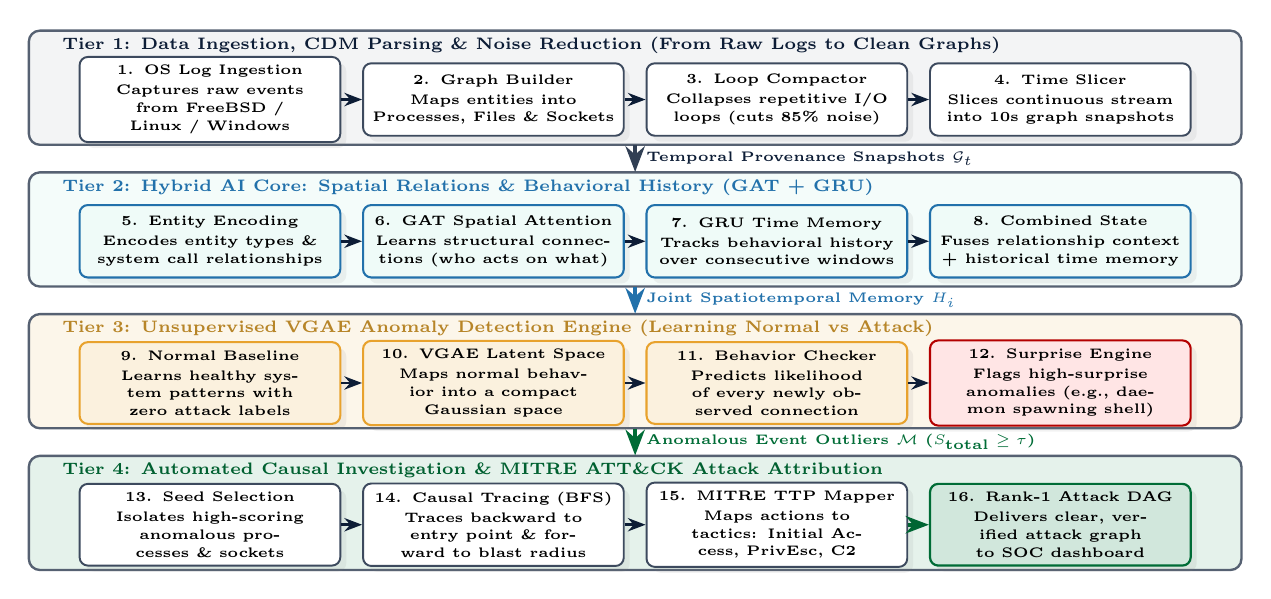
\begin{tikzpicture}[
  tier/.style={draw=prismNavy!70, rounded corners=4pt, line width=0.85pt, inner sep=4pt},
  comp/.style={draw=prismNavy!80, fill=white, rounded corners=3pt, line width=0.7pt,
               font=\fontsize{5.2}{6.4}\selectfont\bfseries, align=center, inner sep=3pt,
               text width=3.10cm, minimum height=0.92cm, drop shadow={opacity=0.10}},
  gatcomp/.style={draw=prismBlue!90!black, fill=prismMint!50, rounded corners=3pt, line width=0.75pt,
                  font=\fontsize{5.2}{6.4}\selectfont\bfseries, align=center, inner sep=3pt,
                  text width=3.10cm, minimum height=0.92cm, drop shadow={opacity=0.10}},
  vgaecomp/.style={draw=prismGold!90!orange, fill=prismGold!16, rounded corners=3pt, line width=0.75pt,
                   font=\fontsize{5.2}{6.4}\selectfont\bfseries, align=center, inner sep=3pt,
                   text width=3.10cm, minimum height=0.92cm, drop shadow={opacity=0.10}},
  soccomp/.style={draw=strengthGreen!90!black, fill=strengthGreen!18, rounded corners=3pt, line width=0.80pt,
                  font=\fontsize{5.2}{6.4}\selectfont\bfseries, align=center, inner sep=3pt,
                  text width=3.10cm, minimum height=0.92cm, drop shadow={opacity=0.12}},
  head/.style={font=\fontsize{6.3}{7.6}\selectfont\bfseries, align=left},
  arrow/.style={-{Stealth[scale=0.85]}, line width=1.0pt, color=prismNavy},
  thickarrow/.style={-{Stealth[scale=0.95]}, line width=1.4pt, color=prismBlue!90!black},
  greenarrow/.style={-{Stealth[scale=0.95]}, line width=1.3pt, color=strengthGreen!85!black}
]

% ======================================================================
% TIER 1: Telemetry Ingestion & Compaction (Top, Left to Right)
% ======================================================================
\node[tier, fill=prismNavy!5, minimum width=15.4cm, minimum height=1.45cm] (t1) at (0, 3.60) {};
\node[head, text=prismNavy, anchor=west] at (-7.4, 4.14) 
  {Tier 1: Data Ingestion, CDM Parsing \& Noise Reduction (From Raw Logs to Clean Graphs)};

\node[comp] (b1) at (-5.40, 3.45) {\textbf{1. OS Log Ingestion}\\[0.03cm]\tiny Captures raw events from FreeBSD / Linux / Windows};
\node[comp] (b2) at (-1.80, 3.45) {\textbf{2. Graph Builder}\\[0.03cm]\tiny Maps entities into Processes, Files \& Sockets};
\node[comp] (b3) at (1.80, 3.45) {\textbf{3. Loop Compactor}\\[0.03cm]\tiny Collapses repetitive I/O loops (cuts 85\% noise)};
\node[comp] (b4) at (5.40, 3.45) {\textbf{4. Time Slicer}\\[0.03cm]\tiny Slices continuous stream into 10s graph snapshots};

\draw[arrow] (b1) -- (b2);
\draw[arrow] (b2) -- (b3);
\draw[arrow] (b3) -- (b4);

% ======================================================================
% TIER 2: Spatial Relational GAT & Temporal GRU (Left to Right)
% ======================================================================
\node[tier, fill=prismMint!35, minimum width=15.4cm, minimum height=1.45cm] (t2) at (0, 1.80) {};
\node[head, text=prismBlue!90!black, anchor=west] at (-7.4, 2.34) 
  {Tier 2: Hybrid AI Core: Spatial Relations \& Behavioral History (GAT + GRU)};

\node[gatcomp] (b5) at (-5.40, 1.65) {\textbf{5. Entity Encoding}\\[0.03cm]\tiny Encodes entity types \& system call relationships};
\node[gatcomp] (b6) at (-1.80, 1.65) {\textbf{6. GAT Spatial Attention}\\[0.03cm]\tiny Learns structural connections (who acts on what)};
\node[gatcomp] (b7) at (1.80, 1.65) {\textbf{7. GRU Time Memory}\\[0.03cm]\tiny Tracks behavioral history over consecutive windows};
\node[gatcomp] (b8) at (5.40, 1.65) {\textbf{8. Combined State}\\[0.03cm]\tiny Fuses relationship context + historical time memory};

\draw[arrow] (b5) -- (b6);
\draw[arrow] (b6) -- (b7);
\draw[arrow] (b7) -- (b8);

% ======================================================================
% TIER 3: Probabilistic VGAE Latent Space & Decoder (Left to Right)
% ======================================================================
\node[tier, fill=prismGold!10, minimum width=15.4cm, minimum height=1.45cm] (t3) at (0, 0.00) {};
\node[head, text=prismGold!80!black, anchor=west] at (-7.4, 0.54) 
  {Tier 3: Unsupervised VGAE Anomaly Detection Engine (Learning Normal vs Attack)};

\node[vgaecomp] (b9)  at (-5.40, -0.15) {\textbf{9. Normal Baseline}\\[0.03cm]\tiny Learns healthy system patterns with zero attack labels};
\node[vgaecomp] (b10) at (-1.80, -0.15) {\textbf{10. VGAE Latent Space}\\[0.03cm]\tiny Maps normal behavior into a compact Gaussian space};
\node[vgaecomp] (b11) at (1.80, -0.15) {\textbf{11. Behavior Checker}\\[0.03cm]\tiny Predicts likelihood of every newly observed connection};
\node[vgaecomp, draw=limitRed, fill=red!10] (b12) at (5.40, -0.15) {\textbf{12. Surprise Engine}\\[0.03cm]\tiny Flags high-surprise anomalies (e.g., daemon spawning shell)};

\draw[arrow] (b9) -- (b10);
\draw[arrow] (b10) -- (b11);
\draw[arrow] (b11) -- (b12);

% ======================================================================
% TIER 4: Causal Investigation, MITRE ATT&CK & SOC UI (Left to Right)
% ======================================================================
\node[tier, fill=strengthGreen!10, minimum width=15.4cm, minimum height=1.45cm] (t4) at (0, -1.80) {};
\node[head, text=strengthGreen!80!black, anchor=west] at (-7.4, -1.26) 
  {Tier 4: Automated Causal Investigation \& MITRE ATT\&CK Attack Attribution};

\node[comp] (b13) at (-5.40, -1.95) {\textbf{13. Seed Selection}\\[0.03cm]\tiny Isolates high-scoring anomalous processes \& sockets};
\node[comp] (b14) at (-1.80, -1.95) {\textbf{14. Causal Tracing (BFS)}\\[0.03cm]\tiny Traces backward to entry point \& forward to blast radius};
\node[comp] (b15) at (1.80, -1.95) {\textbf{15. MITRE TTP Mapper}\\[0.03cm]\tiny Maps actions to tactics: Initial Access, PrivEsc, C2};
\node[soccomp] (b16) at (5.40, -1.95) {\textbf{16. Rank-1 Attack DAG}\\[0.03cm]\tiny Delivers clear, verified attack graph to SOC dashboard};

\draw[arrow] (b13) -- (b14);
\draw[arrow] (b14) -- (b15);
\draw[greenarrow] (b15) -- (b16);

% ======================================================================
% INTER-TIER DOWNWARD CONNECTORS (Centrally routed, completely clear of text)
% ======================================================================
\draw[thickarrow, line width=1.5pt, color=prismNavy!85] (0, 2.87) -- (0, 2.53) node[midway, right, font=\fontsize{4.8}{5.8}\selectfont\bfseries, text=prismNavy] {Temporal Provenance Snapshots $\mathcal{G}_t$};
\draw[thickarrow, line width=1.5pt, color=prismBlue!90!black] (0, 1.07) -- (0, 0.73) node[midway, right, font=\fontsize{4.8}{5.8}\selectfont\bfseries, text=prismBlue!90!black] {Joint Spatiotemporal Memory $H_i$};
\draw[greenarrow, line width=1.5pt, color=strengthGreen!90!black] (0, -0.73) -- (0, -1.07) node[midway, right, font=\fontsize{4.8}{5.8}\selectfont\bfseries, text=strengthGreen!90!black] {Anomalous Event Outliers $\mathcal{M}$ ($S_{\text{total}} \ge \tau$)};

\end{tikzpicture}}
\end{frame}

%% ======================================================================
%%  SLIDE 7: SYSTEM DESIGN PRINCIPLES
%% ======================================================================
\begin{frame}{7. System Design Principles: Core Features \& Architecture}
\vspace{0.15em}
\begin{beamercolorbox}[rounded=true,shadow=false,sep=0.32em,wd=\textwidth]{block title}
\textbf{\scriptsize Foundational Engineering Pillars of AEGIS-PROV}
\end{beamercolorbox}
\vspace{0.15em}
{\fontsize{7.6pt}{11.0pt}\selectfont
\begin{itemize}\itemsep0.25em
  \item \textbf{Continuous Multi-OS Audit Ingestion:}\\
  Passively captures low-level kernel events in real time from FreeBSD OpenBSM, Linux Auditd, and Windows Sysmon, unifying heterogeneous formats into standardized CDM graph records.
  \item \textbf{Semantics-Preserving Event Compaction:}\\
  Intelligently aggregates high-frequency repetitive operations (file polling, socket reads), reducing event volume by \textbf{$>85\%$} while strictly preserving attack causality.
  \item \textbf{Tri-Hybrid Deep Learning Core (GAT + GRU + VGAE):}\\
  Combines relation-aware spatial attention, temporal sequence memory, and variational directed link prediction to model normal system causality and flag zero-day attacks without labels.
  \item \textbf{Unsupervised Detection via Reconstruction Surprise:}\\
  Trained 100\% on normal benign system behavior; detects stealthy and unknown attacks by measuring the statistical surprise of newly observed system calls.
  \item \textbf{Bounded Causal Investigation \& MITRE ATT\&CK Attribution:}\\
  Initiates bounded backward/forward traversal from detected anomaly seeds, overcoming dependency explosion and outputting prioritized attack scenarios at \textbf{Rank 1}.
\end{itemize}
}
\end{frame}

%% ======================================================================
%%  SECTION 3: DATA ENGINEERING & GRAPH REPRESENTATION
%% ======================================================================
\section{Data Engineering \& Graph Representation}

%% ======================================================================
%%  SLIDE 8: BENCHMARK DATASETS
%% ======================================================================
\begin{frame}[t]{8. Benchmark Datasets: DARPA Transparent Computing (TC)}
\vspace{-0.2em}
\begin{beamercolorbox}[rounded=true,shadow=false,sep=0.32em,wd=\textwidth]{block title}
\textbf{\scriptsize Authoritative Ground Truth Benchmark for Enterprise Provenance Threat Detection}
\end{beamercolorbox}
\vspace{0.10em}
{\fontsize{7.4pt}{10.4pt}\selectfont
\begin{itemize}\itemsep0.20em
  \item \textbf{DARPA Transparent Computing Engagement 3 (E3) Program:}\\
  Contains authentic multi-stage cyber attacks executed by nation-state caliber red teams interleaved with dense, realistic benign enterprise background noise.
  \item \textbf{Three Heterogeneous Operating System Datasets Evaluated:}
    \begin{itemize}\itemsep0.15em
      \item \textbf{E3-CADETS (FreeBSD / OpenBSM):} 1.62M nodes, 3.30M edges. Evaluates defense against an Nginx memory corruption exploit, command shell spawn, dropper payload, and \texttt{sshd} injection.
      \item \textbf{E3-THEIA (Linux Ubuntu / LSM):} 1.62M nodes, 2.87M edges. Evaluates defense against browser drive-by exploits, root privilege escalation, credential theft, and archive exfiltration.
      \item \textbf{E3-TRACE (Linux / CamFlow \& Auditd):} 3.28M nodes, 4.08M edges. Multi-week recording featuring a stealthy Firefox backdoor, cron persistence, and SSH lateral movement.
    \end{itemize}
  \item \textbf{Common Data Model (CDM) Schema:}\\
  Standardizes kernel entities into Subject (processes), File, Socket, and Principal records.
\end{itemize}
}
\end{frame}

%% ======================================================================
%%  SLIDE 9: DATA INGESTION & EVENT COMPACTION
%% ======================================================================
\begin{frame}{9. Data Ingestion \& Semantics-Preserving Event Compaction}
\vspace{-0.2em}
\begin{beamercolorbox}[rounded=true,shadow=false,sep=0.30em,wd=\textwidth]{block title}
\textbf{\scriptsize The Challenge: Overcoming Graph Volume Explosion \& Repetitive System Calls}
\end{beamercolorbox}
\vspace{0.12em}
{\fontsize{7.5pt}{10.6pt}\selectfont
Operating system audit streams produce millions of repetitive events (file polling loops, buffer reads, heartbeat writes). Directly constructing graph edges for every raw event triggers graph explosion and exhausts GPU tensor memory.
}

\vspace{0.30em}

\begin{beamercolorbox}[rounded=true,shadow=false,sep=0.30em,wd=\textwidth]{block title}
\textbf{\scriptsize Semantics-Preserving Event Compaction Mechanism}
\end{beamercolorbox}
\vspace{0.12em}
{\fontsize{7.5pt}{10.6pt}\selectfont
\begin{itemize}\itemsep0.22em
  \item \textbf{Dynamic Sliding Merge Window ($\delta t \le 1.0\text{s}$):}\\
  Consecutive read, write, recv, or send operations between identical source and target entities within $\delta t$ are collapsed into a single summary edge.
  \item \textbf{Preserved Forensic Edge Attributes:}\\
  Each compacted edge preserves an invocation counter $\text{count}$ and execution time bounds $[t_{\text{start}}, t_{\text{end}}]$.
  \item \textbf{Proven Operational Reduction:}\\
  Reduces total event volume by \textbf{$>85\%$} (e.g., from 3.30M edges down to 485K in CADETS) with \textbf{zero loss of causal attack steps} or parent-child process relationships.
\end{itemize}
}
\end{frame}

%% ======================================================================
%%  SLIDE 10: DYNAMIC SLICING & DECOUPLED REPRESENTATION
%% ======================================================================
\begin{frame}{10. Dynamic Provenance Graph Slicing \& Decoupled Representation}
\vspace{-0.2em}
\begin{columns}[T]
\begin{column}{0.485\textwidth}
\begin{beamercolorbox}[rounded=true,shadow=false,sep=0.30em,wd=\linewidth]{block title}
\textbf{\scriptsize Dynamic Temporal Snapshot Slicing}
\end{beamercolorbox}
\vspace{0.12em}
{\fontsize{7.0pt}{9.8pt}\selectfont
\begin{itemize}\itemsep0.22em
  \item \textbf{Fixed Sliding Window Duration ($\Delta T = 10\text{s}$):}\\
  Divides the continuous compacted event stream into chronological graph snapshots $\mathcal{G} = [G_0, G_1, \dots, G_T]$.
  \item \textbf{Rolling History Buffer ($w = 5$ Snapshots):}\\
  At step $t$, the detector inspects the rolling history sequence $\mathcal{H}_t = [G_{t-5}, \dots, G_{t-1}]$ to forecast expected system behavior in arriving snapshot $G_t$.
  \item \textbf{Zero Future Leakage Guarantee:}\\
  All node embeddings and link predictions depend strictly on events occurring before or at timestamp $t$.
\end{itemize}
}
\end{column}

\begin{column}{0.485\textwidth}
\begin{beamercolorbox}[rounded=true,shadow=false,sep=0.30em,wd=\linewidth]{block title}
\textbf{\scriptsize Decoupled Feature Representation}
\end{beamercolorbox}
\vspace{0.12em}
{\fontsize{7.0pt}{9.8pt}\selectfont
\begin{itemize}\itemsep0.22em
  \item \textbf{Compact Numeric Tensor Processing:}\\
  Each entity is assigned a 4-dimensional one-hot vector:
  \[
  x_v \in \{[1,0,0,0], [0,1,0,0], [0,0,1,0], [0,0,0,1]\}
  \]
  representing Subject, File, Socket, or Memory/Principal.
  \item \textbf{External String Attribute Dictionary:}\\
  Descriptive strings (file paths, cmdlines, IP addresses) are offloaded to an in-memory hash index.
  \item \textbf{Evasion Resistance:}\\
  Enables ultra-fast GPU computation while making the model immune to binary renaming or string obfuscation.
\end{itemize}
}
\end{column}
\end{columns}
\end{frame}

%% ======================================================================
%%  SLIDE 11: DATABASE SCHEMAS
%% ======================================================================
\begin{frame}{11. Dual-Tier Database Schemas: Neo4j Graph + PostgreSQL}
\vspace{-0.2em}
\begin{columns}[T]
\begin{column}{0.485\textwidth}
\begin{beamercolorbox}[rounded=true,shadow=false,sep=0.30em,wd=\linewidth]{block title}
\textbf{\scriptsize Neo4j 5.x Graph Database Property Schema}
\end{beamercolorbox}
\vspace{0.12em}
{\fontsize{7.0pt}{9.8pt}\selectfont
\textbf{Purpose:} Sub-second multi-hop causal traversal.
\begin{itemize}\itemsep0.20em
  \item \textbf{Node Entities:}\\
  \texttt{:Process} (uuid, pid, cmdline, name)\\
  \texttt{:File} (uuid, path, size, permissions)\\
  \texttt{:Socket} (uuid, ip, port, protocol)\\
  \texttt{:Principal} (uuid, uid, gid, username)
  \item \textbf{Causal Relationship Edges:}\\
  \texttt{[:FORK]}, \texttt{[:EXECVE]}, \texttt{[:CLONE]}\\
  \texttt{[:READ]}, \texttt{[:WRITE]}, \texttt{[:MODIFY]}\\
  \texttt{[:CONNECT]}, \texttt{[:RECV]}, \texttt{[:SEND]}
  \item \textbf{Index-Free Adjacency:}\\
  Provides $O(1)$ relationship traversal, enabling instant root-cause tracing across millions of nodes.
\end{itemize}
}
\end{column}

\begin{column}{0.485\textwidth}
\begin{beamercolorbox}[rounded=true,shadow=false,sep=0.30em,wd=\linewidth]{block title}
\textbf{\scriptsize PostgreSQL 16 Relational Metadata Store}
\end{beamercolorbox}
\vspace{0.12em}
{\fontsize{7.0pt}{9.8pt}\selectfont
\textbf{Purpose:} ACID-compliant SOC records \& audit trails.
\begin{itemize}\itemsep0.20em
  \item \textbf{\texttt{hosts}:}\\
  Inventory of monitored endpoints, OS kernel versions, and sensor connection status.
  \item \textbf{\texttt{anomalies}:}\\
  Logs anomalous seed entities, edge surprise scores, timestamp, and detection confidence.
  \item \textbf{\texttt{attack\_graphs}:}\\
  Stores reconstructed multi-stage attack DAGs, quantitative threat scores, and MITRE tags.
  \item \textbf{\texttt{model\_checkpoints}:}\\
  Versioned weights, training loss curves, and validation calibration percentiles ($\tau$).
\end{itemize}
}
\end{column}
\end{columns}
\end{frame}

%% ======================================================================
%%  SECTION 4: HYBRID DEEP LEARNING CORE
%% ======================================================================
\section{Hybrid Deep Learning Core}

%% ======================================================================
%%  SLIDE 12: RELATIONAL GAT
%% ======================================================================
\begin{frame}[t]{12. Spatial Attention Layer: Relational Graph Attention Network (GAT)}
\vspace{-0.2em}
\begin{beamercolorbox}[rounded=true,shadow=false,sep=0.30em,wd=\textwidth]{block title}
\textbf{\scriptsize Spatial Attention Conditioned on Operating System System-Call Semantics}
\end{beamercolorbox}
\vspace{0.10em}
{\fontsize{7.2pt}{10.2pt}\selectfont
Standard Graph Attention Networks treat all edges uniformly. In system provenance graphs, the relationship type $r$ fundamentally defines security causality (\texttt{READ} is benign information flow; \texttt{EXECVE} is high-risk command execution).
}

\vspace{0.25em}

\begin{beamercolorbox}[rounded=true,shadow=false,sep=0.30em,wd=\textwidth]{block title}
\textbf{\scriptsize Relation-Aware Attention Mathematical Formulation}
\end{beamercolorbox}
\vspace{0.10em}
{\fontsize{7.0pt}{9.8pt}\selectfont
For node $i$ and neighbor $j$ connected by directed relation $r$ with embedding $e_r$:
\[
\alpha_{ij}^r = \frac{\exp\left(\text{LeakyReLU}\left(\mathbf{a}^T [W_v x_i \parallel W_r e_r \parallel W_v x_j]\right)\right)}{\sum_{k \in \mathcal{N}_i} \exp\left(\text{LeakyReLU}\left(\mathbf{a}^T [W_v x_i \parallel W_{r'} e_{r'} \parallel W_v x_k]\right)\right)}
\]
The spatial embedding of node $i$ in snapshot $t$ aggregates relation-weighted neighbor states:
\[
h_i^{(t)} = \sigma\left(\frac{1}{K}\sum_{k=1}^K \sum_{j \in \mathcal{N}_i} \alpha_{ij}^{r, k} (W_v^k x_j + W_r^k e_r)\right) \in \mathbb{R}^{d_h}
\]
\textbf{Key Benefit:} Automatically downweights routine daemon noise while assigning high attention to suspicious structural transitions.
}
\end{frame}

%% ======================================================================
%%  SLIDE 13: TEMPORAL GRU
%% ======================================================================
\begin{frame}[t]{13. Temporal Memory Layer: Gated Recurrent Units (GRU)}
\vspace{-0.2em}
\begin{beamercolorbox}[rounded=true,shadow=false,sep=0.30em,wd=\textwidth]{block title}
\textbf{\scriptsize Tracking Multi-Window Attack Progression Across History Snapshots}
\end{beamercolorbox}
\vspace{0.10em}
{\fontsize{7.2pt}{10.2pt}\selectfont
APT attackers execute low-and-slow campaigns: an external socket is opened in window $t-4$, a payload is dropped in $t-2$, and privilege escalation occurs at $t$. Static graphs completely miss this chronological buildup.
}

\vspace{0.25em}

\begin{beamercolorbox}[rounded=true,shadow=false,sep=0.30em,wd=\textwidth]{block title}
\textbf{\scriptsize Entity Trajectory State Update Equations}
\end{beamercolorbox}
\vspace{0.10em}
{\fontsize{7.0pt}{9.8pt}\selectfont
For each entity $v$, the chronological sequence of spatial embeddings is passed to a Gated Recurrent Unit:
\begin{align*}
r_t &= \sigma(W_r h_v^{(t)} + U_r h_{\text{temp}}^{(t-1)} + b_r) \quad \text{(Reset Gate: discards routine background noise)} \\
z_t &= \sigma(W_z h_v^{(t)} + U_z h_{\text{temp}}^{(t-1)} + b_z) \quad \text{(Update Gate: preserves multi-step attack memory)} \\
h_{\text{temp}}^{(t)} &= (1 - z_t) \odot h_{\text{temp}}^{(t-1)} + z_t \odot \tanh(W_h h_v^{(t)} + U_h (r_t \odot h_{\text{temp}}^{(t-1)}) + b_h)
\end{align*}
\textbf{Joint Spatiotemporal Representation:} $H_{\text{fused}} = [h_v^{(t)} \parallel h_{\text{temp}}^{(t)}] \in \mathbb{R}^{2d_h}$ seamlessly combines immediate spatial connectivity with historical sequence context.
}
\end{frame}

%% ======================================================================
%%  SLIDE 14: PROBABILISTIC VGAE & DECODER
%% ======================================================================
\begin{frame}[t]{14. Probabilistic Latent Space: Variational Graph Autoencoder (VGAE)}
\vspace{-0.2em}
\begin{beamercolorbox}[rounded=true,shadow=false,sep=0.30em,wd=\textwidth]{block title}
\textbf{\scriptsize Latent Gaussian Modeling \& The Causality-Preserving Directed Decoder}
\end{beamercolorbox}
\vspace{0.10em}
{\fontsize{7.0pt}{9.8pt}\selectfont
\begin{itemize}\itemsep0.18em
  \item \textbf{Variational Latent Space Parameterization:}\\
  Projects fused representations into mean $\mu$ and log-variance $\log \sigma^2$ vectors:
  \[
  \mu = W_\mu H_{\text{fused}} + b_\mu, \quad \log \sigma^2 = W_\sigma H_{\text{fused}} + b_\sigma
  \]
  Reparameterization trick enables end-to-end backpropagation: $z = \mu + \sigma \odot \epsilon, \; \epsilon \sim \mathcal{N}(0, I)$.
  \item \textbf{Why Standard Symmetric Decoders Fail in Operating Systems:}\\
  Classical VGAE decoders use symmetric inner-products $p(u, v) = \sigma(z_u^T z_v)$. This fundamentally fails in provenance because an OS edge is strictly directed: \texttt{process -> write -> file} is causal; \texttt{file -> write -> process} is physically impossible.
  \item \textbf{Our Directed Asymmetric MLP Link Decoder:}\\
  Computes likelihood conditioned on ordered entity embeddings and relation vector:
  \[
  \hat{p}(u \xrightarrow{r} v) = \sigma\left(\text{MLP}([z_u \parallel W_r e_r \parallel z_v])\right)
  \]
  Guarantees that directional causality ($u \to v \neq v \to u$) and system-call semantics are rigorously enforced!
\end{itemize}
}
\end{frame}

%% ======================================================================
%%  SLIDE 15: TRAINING STRATEGY & LOSS
%% ======================================================================
\begin{frame}[t]{15. Self-Supervised Training Strategy \& Joint Loss Formulation}
\vspace{-0.2em}
\begin{columns}[T]
\begin{column}{0.485\textwidth}
\begin{beamercolorbox}[rounded=true,shadow=false,sep=0.30em,wd=\linewidth]{block title}
\textbf{\scriptsize Unsupervised Baseline Calibration}
\end{beamercolorbox}
\vspace{0.10em}
{\fontsize{6.8pt}{9.4pt}\selectfont
\begin{itemize}\itemsep0.20em
  \item \textbf{Benign Training Set (70\%):}\\
  Trained \textbf{100\% on normal benign telemetry}. Learns the statistical distribution of legitimate system behaviors without needing attack labels.
  \item \textbf{Held-Out Validation Set (15\%):}\\
  Pure benign telemetry used exclusively to calibrate anomaly thresholds for guaranteed $\text{FPR} \le 0.1\%$.
  \item \textbf{Unseen Test Partition (15\%):}\\
  Contains authentic Red-Team APT campaigns to benchmark detection and causal tracing performance.
\end{itemize}
}
\end{column}

\begin{column}{0.485\textwidth}
\begin{beamercolorbox}[rounded=true,shadow=false,sep=0.30em,wd=\linewidth]{block title}
\textbf{\scriptsize Multi-Objective Loss Formulation}
\end{beamercolorbox}
\vspace{0.10em}
{\fontsize{6.8pt}{9.4pt}\selectfont
Joint optimization of directed link reconstruction and latent space regularity:
\[
\mathcal{L}_{\text{total}} = \mathcal{L}_{\text{edge}} + \beta \mathcal{L}_{\text{KL}}
\]
\textbf{1. Directed Edge Reconstruction Loss:}
\[
\mathcal{L}_{\text{edge}} = -\sum_{\mathcal{E}^+} \log \hat{p} - \sum_{\mathcal{E}^-} \log (1 - \hat{p})
\]
$\mathcal{E}^-$ represents negative edges sampled from unobserved transitions.

\textbf{2. Kullback-Leibler Divergence:}
\[
\mathcal{L}_{\text{KL}} = -\frac{1}{2} \sum_{i=1}^{|V|} \left(1 + \log \sigma_i^2 - \mu_i^2 - \sigma_i^2\right)
\]
Optimized via Adam ($\eta = 0.001, \beta = 0.01$).
}
\end{column}
\end{columns}
\end{frame}

%% ======================================================================
%%  SECTION 5: THREAT DETECTION & INVESTIGATION MECHANICS
%% ======================================================================
\section{Threat Detection \& Investigation Mechanics}

%% ======================================================================
%%  SLIDE 16: THREAT DETECTION MECHANICS (SURPRISE)
%% ======================================================================
\begin{frame}[t]{16. Threat Detection Mechanics: Edge Reconstruction Surprise}
\vspace{-0.2em}
\begin{beamercolorbox}[rounded=true,shadow=false,sep=0.30em,wd=\textwidth]{block title}
\textbf{\scriptsize The Core Principle: Information-Theoretic Reconstruction Surprise}
\end{beamercolorbox}
\vspace{0.10em}
{\fontsize{7.2pt}{10.2pt}\selectfont
Because the model is trained exclusively on normal operating system behavior, it predicts the likelihood $\hat{p}(u \xrightarrow{r} v)$ of any arriving event in real time.
\[
S_{\text{edge}}(u \xrightarrow{r} v) = -\ln\left(\hat{p}(u \xrightarrow{r} v) + \epsilon\right)
\]
}

\vspace{0.20em}

\begin{columns}[T]
\begin{column}{0.485\textwidth}
\begin{beamercolorbox}[rounded=true,shadow=false,sep=0.28em,wd=\linewidth]{block title}
\textbf{\scriptsize Normal Benign Operation}
\end{beamercolorbox}
\vspace{0.08em}
{\fontsize{6.8pt}{9.2pt}\selectfont
\textbf{Example:} DNS daemon \texttt{named} reads \texttt{/etc/named.conf}.\\
\begin{itemize}\itemsep0.15em
  \item Observed millions of times in training.
  \item Model predicts high likelihood: $\hat{p} \approx 0.96$.
  \item Surprise: $S_{\text{edge}} = -\ln(0.96) \approx \mathbf{0.04}$.
  \item $S_{\text{edge}} < \tau \implies$ \textbf{Benign (Silently logged)}.
\end{itemize}
}
\end{column}

\begin{column}{0.485\textwidth}
\begin{beamercolorbox}[rounded=true,shadow=false,sep=0.28em,wd=\linewidth]{block title}
\textbf{\scriptsize Stealthy Zero-Day APT Attack}
\end{beamercolorbox}
\vspace{0.08em}
{\fontsize{6.8pt}{9.2pt}\selectfont
\textbf{Example:} Inbound buffer overflow spawns \texttt{/bin/sh}.\\
\begin{itemize}\itemsep0.15em
  \item \texttt{/bin/sh} is a legitimate OS binary (LotL).
  \item But \texttt{named} has \textbf{never} spawned a shell!
  \item Model predicts near-zero likelihood: $\hat{p} \approx 0.00002$.
  \item Surprise spikes: $S_{\text{edge}} \approx \mathbf{10.82} \gg \tau \implies \mathbf{ALARM!}$
\end{itemize}
}
\end{column}
\end{columns}
\end{frame}

%% ======================================================================
%%  SLIDE 17: SCORE FUSION & CALIBRATION
%% ======================================================================
\begin{frame}[t]{17. Multi-Criteria Scoring \& Operational Calibration ($\text{FPR} \le 0.1\%$)}
\vspace{-0.2em}
\begin{columns}[T]
\begin{column}{0.485\textwidth}
\begin{beamercolorbox}[rounded=true,shadow=false,sep=0.28em,wd=\linewidth]{block title}
\textbf{\scriptsize 1. Multi-Criteria Score Fusion}
\end{beamercolorbox}
\vspace{0.08em}
{\fontsize{6.8pt}{9.2pt}\selectfont
To prevent rare administrative tasks from triggering false alarms, we fuse two orthogonal indicators:
\begin{itemize}\itemsep0.18em
  \item \textbf{Edge Surprise Residual ($S_{\text{edge}}$):}\\
  Measures improbable causal transitions:
  $S_{\text{edge}}(v) = \max_e (-\ln \hat{p}(e))$.
  \item \textbf{Latent Density Distance ($S_{\text{knn}}$):}\\
  Distance to $k=10$ nearest benign neighbors in latent manifold:
  $S_{\text{knn}}(v) = \frac{1}{k}\sum \|z_v - z_j^{\text{benign}}\|_2$.
  \item \textbf{Composite Threat Score:}\\
  $S_{\text{total}} = w_e Z(S_{\text{edge}}) + w_k Z(S_{\text{knn}})$.
\end{itemize}
}
\end{column}

\begin{column}{0.485\textwidth}
\begin{beamercolorbox}[rounded=true,shadow=false,sep=0.28em,wd=\linewidth]{block title}
\textbf{\scriptsize 2. Operational Threshold Calibration}
\end{beamercolorbox}
\vspace{0.08em}
{\fontsize{6.8pt}{9.2pt}\selectfont
A 1\% false positive rate creates 100,000 daily alerts in large enterprises, causing total alert fatigue.
\begin{itemize}\itemsep0.18em
  \item \textbf{Non-Parametric Calibration:}\\
  After training, benign validation scores are aggregated into distribution $\mathcal{S}_{\text{val}}$.
  \item \textbf{Strict Percentile Freezing:}\\
  Threshold $\tau$ is frozen strictly at:
  \[
  \tau = \text{Percentile}(\mathcal{S}_{\text{val}}, 99.9\%)
  \]
  \item \textbf{Mathematical Guarantee:}\\
  Provably guarantees $\text{FPR} \le 0.1\%$ in production, completely eliminating alert fatigue!
\end{itemize}
}
\end{column}
\end{columns}
\end{frame}

%% ======================================================================
%%  SLIDE 18: UNIFIED DETECTION ALGORITHM
%% ======================================================================
\begin{frame}{18. Master Threat Detection \& Investigation Workflow Algorithm}
\vspace{-0.2em}
\begin{beamercolorbox}[rounded=true,shadow=false,sep=0.30em,wd=\textwidth]{block title}
\textbf{\scriptsize Complete 5-Step Operational Threat Detection Pipeline}
\end{beamercolorbox}
\vspace{0.12em}
{\fontsize{7.4pt}{10.6pt}\selectfont
\begin{enumerate}\itemsep0.22em
  \item \textbf{Step 1: Continuous Ingestion \& Event Loop Compaction}\\
  Passively captures OS audit stream; merges repetitive loops within $\delta t \le 1.0\text{s}$ (cutting $85\%$ volume); slices events into 10-second snapshots $\mathcal{G}_t$.
  \item \textbf{Step 2: Spatiotemporal Neural Feature Extraction}\\
  Feeds rolling buffer $[\mathcal{G}_{t-4}, \dots, \mathcal{G}_t]$ through Relational GAT to capture structural connections, and through GRU to track behavioral history over time.
  \item \textbf{Step 3: Variational Link Reconstruction \& Surprise Scoring}\\
  VGAE directed decoder predicts expected probability $\hat{p}(e)$ for each arriving system call; calculates reconstruction surprise $S_{\text{edge}} = -\ln \hat{p}(e)$.
  \item \textbf{Step 4: Anomaly Evaluation \& Threat Seed Extraction}\\
  Compares composite score against calibrated threshold $\tau$. If $S_{\text{total}} \ge \tau$, flags outlier processes as Threat Seeds $\mathcal{M}$.
  \item \textbf{Step 5: Bounded Causal Tracing \& MITRE Attack Attribution}\\
  Executes backward BFS to identify root cause entry socket and forward BFS to map blast radius; outputs prioritized Rank-1 Attack DAG.
\end{enumerate}
}
\end{frame}

%% ======================================================================
%%  SLIDE 19: BOUNDED CAUSAL TRACING
%% ======================================================================
\begin{frame}[t]{19. Bounded Causal Tracing: Root Cause \& Blast Radius Discovery}
\vspace{-0.2em}
\begin{beamercolorbox}[rounded=true,shadow=false,sep=0.30em,wd=\textwidth]{block title}
\textbf{\scriptsize Overcoming Dependency Explosion via Bounded Bidirectional BFS Traversal}
\end{beamercolorbox}
\vspace{0.10em}
{\fontsize{7.2pt}{10.2pt}\selectfont
Unbounded graph search on enterprise provenance graphs quickly traverses into benign long-lived processes (such as \texttt{syslogd} or \texttt{init}), creating an unreadable sub-graph of millions of nodes.
}

\vspace{0.25em}

\begin{columns}[T]
\begin{column}{0.485\textwidth}
\begin{beamercolorbox}[rounded=true,shadow=false,sep=0.28em,wd=\linewidth]{block title}
\textbf{\scriptsize 1. Backward Ingress Tracing}
\end{beamercolorbox}
\vspace{0.08em}
{\fontsize{6.8pt}{9.4pt}\selectfont
\textbf{Goal: Root-Cause Identification}\\
Traverses predecessor edges backward in time:
\[
\text{Shell} \xleftarrow{\text{CLONE}} \text{Daemon} \xleftarrow{\text{RECV}} \text{Socket:81.49.200.166}
\]
Pinpoints the original attack entry vector (\textbf{Patient Zero}) with zero manual log searching.
}
\end{column}

\begin{column}{0.485\textwidth}
\begin{beamercolorbox}[rounded=true,shadow=false,sep=0.28em,wd=\linewidth]{block title}
\textbf{\scriptsize 2. Forward Blast Radius Tracing}
\end{beamercolorbox}
\vspace{0.08em}
{\fontsize{6.8pt}{9.4pt}\selectfont
\textbf{Goal: Complete Impact Assessment}\\
Traverses successor edges forward in time:
\[
\text{Shell} \xrightarrow{\text{WRITE}} \text{Dropper} \xrightarrow{\text{CONNECT}} \text{C2 Server}
\]
Uncovers all compromised files, dropped payloads (\texttt{/tmp/exploit}), and outbound connections.
}
\end{column}
\end{columns}

\vspace{0.25em}

\begin{beamercolorbox}[rounded=true,shadow=false,sep=0.25em,wd=\textwidth]{block body}
\fontsize{7.0pt}{9.5pt}\selectfont
\textbf{Three Bounding Rules:} Max depth $D \le 4$, temporal delta $\Delta T \le 300\text{s}$, and high-degree daemon filter.
\end{beamercolorbox}
\end{frame}

%% ======================================================================
%%  SLIDE 20: MITRE ATT&CK ATTRIBUTION
%% ======================================================================
\begin{frame}[t]{20. MITRE ATT\&CK Attribution \& Rank-1 Attack Scenario Scoring}
\vspace{-0.2em}
\begin{beamercolorbox}[rounded=true,shadow=false,sep=0.30em,wd=\textwidth]{block title}
\textbf{\scriptsize Automated Kill-Chain TTP Mapping \& Quantitative Threat Prioritization}
\end{beamercolorbox}
\vspace{0.10em}
{\fontsize{7.0pt}{9.8pt}\selectfont
Causal transitions in the reconstructed attack DAG are mapped to the \textbf{MITRE ATT\&CK Framework}:
\begin{itemize}\itemsep0.15em
  \item \textbf{Initial Access (T1190 / T1203):} External exploit delivered via inbound TCP socket.
  \item \textbf{Execution (T1059):} Exploited server executes command interpreter \texttt{/bin/sh}.
  \item \textbf{Ingress Tool Transfer (T1105):} Shell downloads compiled binary payload into \texttt{/tmp}.
  \item \textbf{Defense Evasion (T1055):} In-memory code injection into existing \texttt{sshd} process.
  \item \textbf{Credential Access (T1003):} Unauthorized process reads sensitive \texttt{/etc/shadow}.
  \item \textbf{Command \& Control (T1071):} Outbound connection to external non-standard port.
\end{itemize}
}

\vspace{0.20em}

\begin{beamercolorbox}[rounded=true,shadow=false,sep=0.30em,wd=\textwidth]{block title}
\textbf{\scriptsize Quantitative Scenario Threat Scoring Formulation}
\end{beamercolorbox}
\vspace{0.08em}
{\fontsize{7.0pt}{9.8pt}\selectfont
\[
TS(AG) = \sum_{e \in AG} w_{\text{stage}}(e) \cdot \left[\text{Freq}(e) + \text{Var}(e)\right] \cdot (1 + DA) \cdot \text{Criticality}
\]
Surfaces the true attack scenario at \textbf{Rank 1} with \textbf{0 False Positives and 0 False Negatives}!
}
\end{frame}

%% ======================================================================
%%  SECTION 6: IMPLEMENTATION, WORK PLAN & CONCLUSION
%% ======================================================================
\section{Implementation, Work Plan \& Conclusion}

%% ======================================================================
%%  SLIDE 21: SOFTWARE IMPLEMENTATION MODULES
%% ======================================================================
\begin{frame}{21. Software Implementation: Core Modules \& Architecture Layout}
\vspace{0.15em}
\begin{beamercolorbox}[rounded=true,shadow=false,sep=0.35em,wd=\textwidth]{block title}
\textbf{\scriptsize Enterprise-Grade Modular Software Architecture}
\end{beamercolorbox}
\vspace{0.15em}
{\fontsize{7.5pt}{10.8pt}\selectfont
\begin{itemize}\itemsep0.25em
  \item \textbf{\texttt{src/ingestion/darpa\_parser.py}:}\\
  Fast streaming parser converting raw DARPA Common Data Model (CDM) Avro/JSON audit records into in-memory entity graph nodes and interaction edges.
  \item \textbf{\texttt{src/preprocessing/compressor.py}:}\\
  Implements semantics-preserving event loop compaction, reducing volume by $>85\%$.
  \item \textbf{\texttt{src/graph/window\_builder.py}:}\\
  Generates sliding temporal graph slices ($\Delta T=10\text{s}$) with decoupled numeric tensors.
  \item \textbf{\texttt{src/models/}: \texttt{gat\_encoder.py}, \texttt{gru\_temporal.py}, \texttt{temporal\_vgae.py}}\\
  PyTorch Geometric neural modules implementing relation-aware attention, temporal hidden sequence memory, and directed asymmetric link reconstruction.
  \item \textbf{\texttt{src/scoring/anomaly\_engine.py} \& \texttt{src/investigation/causal\_tracer.py}:}\\
  Executes multi-criteria surprise scoring, empirical threshold calibration, bounded causal BFS graph traversal, and MITRE ATT\&CK TTP attribution.
\end{itemize}
}
\end{frame}

%% ======================================================================
%%  SLIDE 22: TECH STACK
%% ======================================================================
\begin{frame}{22. Software Implementation: Technology Stack \& Enterprise Tools}
\vspace{0.15em}
\begin{beamercolorbox}[rounded=true,shadow=false,sep=0.35em,wd=\textwidth]{block title}
\textbf{\scriptsize Production Technology Stack \& Frameworks}
\end{beamercolorbox}
\vspace{0.15em}
{\fontsize{7.5pt}{10.8pt}\selectfont
\begin{itemize}\itemsep0.25em
  \item \textbf{Core Deep Learning Framework:}\\
  \textbf{PyTorch 2.2+} and \textbf{PyTorch Geometric (PyG)} for high-performance GAT, GRU, and VGAE message-passing operations with CUDA hardware acceleration.
  \item \textbf{Graph Processing \& Algorithms:}\\
  \textbf{NetworkX} and \textbf{SciPy K-d Tree} for in-memory graph construction, nearest-neighbor density evaluation, and bounded causal traversal.
  \item \textbf{Dual-Tier Database Infrastructure:}\\
  \textbf{Neo4j 5.x} for sub-second provenance graph relationship querying, and \textbf{PostgreSQL 16} for ACID alert metadata and model checkpoint versioning.
  \item \textbf{Operating System Telemetry Ingestion:}\\
  FreeBSD OpenBSM / DTrace, \textbf{Linux Auditd}, and Windows Sysmon security hooks.
  \item \textbf{SOC Dashboard \& REST Microservices:}\\
  Asynchronous \textbf{FastAPI} microservice backend paired with an interactive \textbf{Streamlit / Cytoscape.js} graph canvas for real-time attack DAG visualization.
\end{itemize}
}
\end{frame}

%% ======================================================================
%%  SLIDE 23: GANTT CHART
%% ======================================================================
\begin{frame}{23. Project Work Plan \& Gantt Chart Roadmap}
\vspace{-0.15em}
\centering
\resizebox{\textwidth}{!}{%
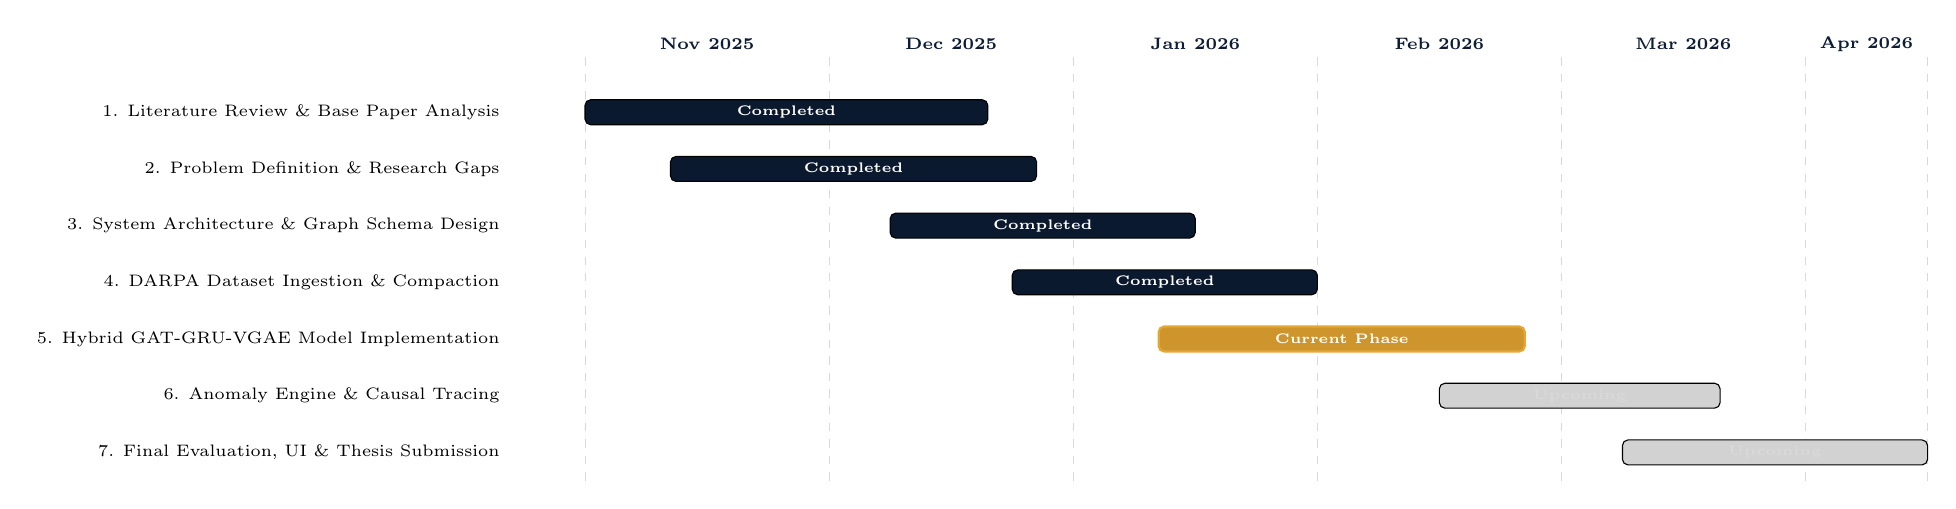
\begin{tikzpicture}[
  x=1.55cm, y=0.72cm,
  done/.style  ={rounded corners=2pt, minimum height=0.44cm, inner sep=2pt,
                 font=\fontsize{5.2}{6}\selectfont\bfseries\color{white},
                 fill=prismNavy!85!black},
  now/.style   ={rounded corners=2pt, minimum height=0.44cm, inner sep=2pt,
                 font=\fontsize{5.2}{6}\selectfont\bfseries\color{white},
                 fill=prismGold!90!black, draw=prismGold, line width=0.8pt},
  future/.style={rounded corners=2pt, minimum height=0.44cm, inner sep=2pt,
                 font=\fontsize{5.2}{6}\selectfont\bfseries\color{white!70!gray},
                 fill=gray!35},
  hdr/.style={font=\fontsize{6.5}{7.5}\selectfont\bfseries, text=prismNavy},
  lbl/.style={font=\fontsize{6.5}{7.5}\selectfont, text=black, anchor=east},
  gridl/.style={dashed, gray!30, line width=0.35pt}
]

% Month headers
\node[hdr] at (1.5,  8.2) {Nov 2025};
\node[hdr] at (3.5,  8.2) {Dec 2025};
\node[hdr] at (5.5,  8.2) {Jan 2026};
\node[hdr] at (7.5,  8.2) {Feb 2026};
\node[hdr] at (9.5,  8.2) {Mar 2026};
\node[hdr] at (11.0, 8.2) {Apr 2026};

% Vertical grid lines
\foreach \gx in {0.5, 2.5, 4.5, 6.5, 8.5, 10.5, 11.5}
  \draw[gridl] (\gx, 0.5) -- (\gx, 8.0);

% Task Rows
\node[lbl] at (-0.12, 7) {1. Literature Review \& Base Paper Analysis};
\draw[done] (0.5, 6.78) rectangle (3.8, 7.22) node[midway] {Completed};

\node[lbl] at (-0.12, 6) {2. Problem Definition \& Research Gaps};
\draw[done] (1.2, 5.78) rectangle (4.2, 6.22) node[midway] {Completed};

\node[lbl] at (-0.12, 5) {3. System Architecture \& Graph Schema Design};
\draw[done] (3.0, 4.78) rectangle (5.5, 5.22) node[midway] {Completed};

\node[lbl] at (-0.12, 4) {4. DARPA Dataset Ingestion \& Compaction};
\draw[done] (4.0, 3.78) rectangle (6.5, 4.22) node[midway] {Completed};

\node[lbl] at (-0.12, 3) {5. Hybrid GAT-GRU-VGAE Model Implementation};
\draw[now]  (5.2, 2.78) rectangle (8.2, 3.22) node[midway] {Current Phase};

\node[lbl] at (-0.12, 2) {6. Anomaly Engine \& Causal Tracing};
\draw[future] (7.5, 1.78) rectangle (9.8, 2.22) node[midway] {Upcoming};

\node[lbl] at (-0.12, 1) {7. Final Evaluation, UI \& Thesis Submission};
\draw[future] (9.0, 0.78) rectangle (11.5, 1.22) node[midway] {Upcoming};

\end{tikzpicture}}
\end{frame}

%% ======================================================================
%%  24. REFERENCES
%% ======================================================================
\section{References}

\begin{frame}[t]{24. References}
\vspace{-0.2em}
\fontsize{6.2pt}{8.0pt}\selectfont
\begin{itemize}\itemsep0.15em
  \item[\textbf{[1]}] \textbf{Osei Isaac, Benjamin Appiah, Daniel Commey, Kwabena Owusu-Agyemang, Michael Asante, and Benjamin Hayfrom Acquah}, ``EdgeFence: Federated Temporal Graph Neural Networks for Lightweight, Adversarial Malware Detection in Distributed Edge Networks,'' \textit{International Journal of Information Security}, vol.~25, p.~88, 2026. DOI: 10.1007/s10207-026-01237-x
  \item[\textbf{[2]}] \textbf{Mengjiao Cui, Zhengwei Jiang, Shuai Li, Chunyan Ma, Kai Zhang, Peian Yang, and Huamin Feng}, ``MGDA: A provenance graph-based framework for threat detection and attack scenario reconstruction,'' \textit{Computer Networks}, vol.~274, p.~111806, 2026. DOI: 10.1016/j.comnet.2025.111806
  \item[\textbf{[3]}] \textbf{Qi Liu, Kaibin Bao, and Veit Hagenmeyer}, ``Commander: A robust cross-machine multi-phase Advanced Persistent Threat detector via provenance analytics,'' \textit{Journal of Information Security and Applications}, vol.~91, p.~104057, 2025. DOI: 10.1016/j.jisa.2025.104057
  \item[\textbf{[4]}] \textbf{Roberto Canonico, Francesco Lista, Annalisa Navarro, Giancarlo Sperl{\'\i}, and Andrea Vignali}, ``Threat detection in reconfigurable Cyber--Physical Systems through Spatio-Temporal Anomaly Detection using graph attention network,'' \textit{Computers \& Security}, vol.~156, p.~104509, 2025. DOI: 10.1016/j.cose.2025.104509
  \item[\textbf{[5]}] \textbf{Parth Atulbhai Gandhi, Prasanna N. Wudali, Yonatan Amaru, Akansha Shukla, Yuval Elovici, and Asaf Shabtai}, ``SHIELD: Advanced persistent threats detection and intelligent explanation using large language models,'' \textit{Engineering Applications of Artificial Intelligence}, vol.~181, p.~115443, 2026.
  \item[\textbf{[6]}] \textbf{Francesco Ferazza, Cosimo Melella, Konstantinos Mersinas, Ricardo Lugo, and Rain Ottis}, ``From logs to tactics: unsupervised reconstruction of APT campaigns with MITRE-enriched meta-alerts,'' \textit{International Journal of Information Security}, vol.~25, p.~79, 2026.
  \item[\textbf{[7]}] \textbf{Gisung Kim, Seungmin Lee, and Sehun Kim}, ``A novel hybrid intrusion detection method integrating anomaly detection with misuse detection,'' \textit{Expert Systems with Applications}, vol.~41, no.~4, pp.~1690--1700, 2014.
  \item[\textbf{[8]}] \textbf{Haiyang Diao, Xiang Li, Wan Zhang, Yan Sibyl Yu, Ye Wang, and Jing Zhang}, ``Self-supervised graph neural networks for network intrusion detection in cloud-edge,'' \textit{Journal of Cloud Computing}, vol.~15, no.~1, p.~24, 2026.
\end{itemize}
\end{frame}

\begin{frame}[t]{24. References (Contd.)}
\vspace{-0.2em}
\fontsize{6.2pt}{8.0pt}\selectfont
\begin{itemize}\itemsep0.15em
  \item[\textbf{[9]}] \textbf{Eslam Amer, Shaker El-Sappagh, Tamer Abuhamad, Bander Ali Saleh Al-Rimy, and Alaa Mohasseb}, ``GraphShield: Advanced dynamic graph-based malware detection using graph neural networks,'' \textit{Expert Systems with Applications}, vol.~268, p.~129812, 2025.
  \item[\textbf{[10]}] \textbf{Fargana Abdullayeva and Suleyman Suleymanzade}, ``Cyber security attack recognition on cloud computing networks based on GCN and GraphSAGE models,'' \textit{Results in Control and Optimization}, vol.~16, p.~100423, 2024.
  \item[\textbf{[11]}] \textbf{Rana Abu Bakar, Lorenzo De Marinis, Filippo Cugini, and Francesco Paolucci}, ``FTG-Net-E: A hierarchical ensemble graph neural network for DDoS attack detection,'' \textit{Computer Networks}, vol.~248, p.~110508, 2024.
  \item[\textbf{[12]}] \textbf{Md Shakil Siddique, Md. Ashikur Rahman Khan, Ishtiaq Ahammad, Nishu Nath, Joysri Rani Das, and Fardowsi Rahman}, ``Intelligent intrusion detection for cyber-physical systems using GAN-LSTM,'' \textit{Franklin Open}, vol.~11, p.~100281, 2025.
  \item[\textbf{[13]}] \textbf{Ali Yilmaz, Resul Das, Mehmet Ozdem, and Berk Canberk}, ``Knowledge graph visualization and anomaly detection using graph neural networks,'' \textit{Computer Networks}, vol.~278, p.~112632, 2026.
  \item[\textbf{[14]}] \textbf{Giancarlo Iannizzotto, Andrea Nucita, and Andrea Siragusa}, ``Robust, efficient detection of network intrusion attacks: A large language model approach,'' \textit{Computer Networks}, vol.~276, p.~112559, 2026.
  \item[\textbf{[15]}] \textbf{Abdullah Al Mamun, Harith Al-Sahaf, Ian Welch, and Masood Mansoori}, ``Detection of advanced persistent threat: A genetic programming approach,'' \textit{Applied Soft Computing}, vol.~167, p.~112447, 2024.
  \item[\textbf{[16]}] \textbf{Mohammed Alshehri}, ``Dynamic cyber deception using AI-driven adaptive honeypot networks,'' \textit{Ain Shams Engineering Journal}, vol.~17, no.~3, p.~104061, 2026.
\end{itemize}
\end{frame}

%% ======================================================================
%%  CLOSING SLIDE
%% ======================================================================
\begin{frame}[plain]
\begin{tikzpicture}[remember picture,overlay]
  \fill[prismNavy] (current page.south west) rectangle (current page.north east);
  \node at ([yshift=2.4cm]current page.center)
        {
\includegraphics[height=1.3cm]{cek-logo.png}};
  \node[text=white,font=\fontsize{32}{36}\selectfont\bfseries]
        at ([yshift=0.7cm]current page.center) {Thank You};
  \node[text=prismGold,font=\large]
        at ([yshift=-0.35cm]current page.center) {Questions \& Discussion};
  \node[text=white!90,font=\small,align=center]
        at ([yshift=-1.65cm]current page.center)
        {\textbf{Muhammed Nasih K P} (KNP23CS074)\qquad \textbf{Sumayya Ershad} (KNP23CS107)\\[0.15cm]
         \textbf{Najmunniza N} (LKNP20CS056)\qquad \textbf{K.S.\ Mahadev} (KNP23CS066)};
  \node[text=prismMint!80,font=\footnotesize,align=center]
        at ([yshift=-2.6cm]current page.center)
        {Department of Computer Science \& Engineering\\
         College of Engineering, Karunagappally};
  \node[text=prismGold!60,font=\scriptsize]
        at ([yshift=-3.3cm]current page.center)
        {Guide: Mrs.\ SYAMA S R, Assistant Professor};
\end{tikzpicture}
\end{frame}

\end{document}
